% ============================================================
%  TP-SAPU: Temporal Parallel Spiking Adaptive Processing Units
%  26-slide Beamer presentation — revised structure
% ============================================================
\documentclass[aspectratio=169,11pt]{beamer}

\usetheme{Madrid}
\usecolortheme{seahorse}
\usefonttheme{professionalfonts}

\usepackage{booktabs}
\usepackage{array}
\usepackage{colortbl}
\usepackage{tikz}
\usetikzlibrary{arrows.meta,positioning,shapes.geometric,fit,backgrounds,calc}
\usepackage{pgfplots}
\pgfplotsset{compat=1.18}
\usepackage{amsmath,amssymb}
\usepackage{graphicx}
\usepackage{xcolor}
\usepackage{multirow}
\usepackage{makecell}
\usepackage{tcolorbox}
\tcbuselibrary{skins,breakable}

% ── palette ──────────────────────────────────────────────────────────────────
\definecolor{accent0}{HTML}{E07B39}
\definecolor{accent1}{HTML}{4C9BE8}
\definecolor{accent2}{HTML}{6BBF59}
\definecolor{darkbg}{HTML}{1E2132}
\definecolor{midbg}{HTML}{2C2F45}
\definecolor{lighttext}{HTML}{EEF0F8}
\definecolor{subtletext}{HTML}{9BA3C0}
\definecolor{highlight}{HTML}{FFD166}
\definecolor{warnred}{HTML}{FF6B6B}

\setbeamercolor{palette primary}{bg=darkbg,fg=lighttext}
\setbeamercolor{palette secondary}{bg=midbg,fg=lighttext}
\setbeamercolor{palette tertiary}{bg=darkbg,fg=lighttext}
\setbeamercolor{palette quaternary}{bg=darkbg,fg=lighttext}
\setbeamercolor{background canvas}{bg=darkbg}
\setbeamercolor{normal text}{fg=lighttext}
\setbeamercolor{frametitle}{bg=midbg,fg=lighttext}
\setbeamercolor{title}{fg=highlight}
\setbeamercolor{subtitle}{fg=accent1}
\setbeamercolor{block title}{bg=accent1!30!midbg,fg=lighttext}
\setbeamercolor{block body}{bg=midbg!70,fg=lighttext}
\setbeamercolor{block title alerted}{bg=accent0!40!midbg,fg=lighttext}
\setbeamercolor{block body alerted}{bg=midbg!70,fg=lighttext}
\setbeamercolor{block title example}{bg=accent2!30!midbg,fg=lighttext}
\setbeamercolor{block body example}{bg=midbg!70,fg=lighttext}
\setbeamercolor{itemize item}{fg=accent1}
\setbeamercolor{itemize subitem}{fg=accent0}
\setbeamercolor{enumerate item}{fg=highlight}
\setbeamercolor{structure}{fg=accent1}

\setbeamertemplate{navigation symbols}{}
\setbeamertemplate{footline}[frame number]
\setbeamertemplate{frametitle}[default][center]
\setbeamertemplate{itemize item}{\textbullet}
\setbeamertemplate{itemize subitem}{\small$\triangleright$}

\newcommand{\hl}[1]{{\color{highlight}\textbf{#1}}}
\newcommand{\blue}[1]{{\color{accent1}#1}}
\newcommand{\orange}[1]{{\color{accent0}#1}}
\newcommand{\green}[1]{{\color{accent2}#1}}
\newcommand{\red}[1]{{\color{warnred}#1}}
\newcommand{\tpsapu}{\textsc{tp-sapu}}
\newcommand{\lif}{\textsc{lif}}

\tcbset{mybox/.style={
  enhanced,
  arc=3pt,
  colback=midbg,
  colframe=accent1!60,
  coltext=lighttext,
  fontupper=\color{lighttext},
  fontlower=\color{lighttext},
  fonttitle=\bfseries\small,
  coltitle=lighttext,
  boxrule=0.5pt,
  left=4pt,
  right=4pt,
  top=3pt,
  bottom=3pt
}}

\tcbset{failbox/.style={
  enhanced,
  arc=3pt,
  colback=midbg,
  colframe=warnred!70,
  coltext=lighttext,
  fontupper=\color{lighttext},
  fontlower=\color{lighttext},
  fonttitle=\bfseries\small,
  coltitle=lighttext,
  boxrule=0.8pt,
  left=4pt,
  right=4pt,
  top=3pt,
  bottom=3pt
}}

\title{\tpsapu: Temporal Parallel Spiking\\Adaptive Processing Units}
\subtitle{Architecture \textbullet{} MNIST \textbullet{} ImageNet \textbullet{} Future Directions}
\author{Mateusz}
\date{June 2026}

% =============================================================================
\begin{document}
% =============================================================================

% ── SLIDE 1: Title ───────────────────────────────────────────────────────────
\begin{frame}[plain]
\begin{tikzpicture}[remember picture,overlay]
  \fill[darkbg] (current page.south west) rectangle (current page.north east);
  \fill[accent1!10,opacity=0.4] (current page.south west)
        .. controls +(3,4) and +(-3,-2) .. (current page.north east);
\end{tikzpicture}
\vspace{0.9cm}
\begin{center}
  {\color{highlight}\fontsize{28}{32}\selectfont\textbf{\tpsapu{}}}\\[0.3em]
  {\color{accent1}\large Temporal Parallel Spiking Adaptive Processing Units}\\[0.8em]
  \textcolor{subtletext}{\rule{0.5\textwidth}{0.4pt}}\\[0.6em]
  {\color{lighttext}\small
    Architecture~$\cdot$~MNIST sanity check~$\cdot$~Tiny ImageNet~$\cdot$~Attention analysis~$\cdot$~Future hardware}\\[0.8em]
  {\color{subtletext}\small Mateusz \quad|\quad June 2026}
\end{center}
\end{frame}

% ── SLIDE 2: Motivation — SNN vs RNN vs CNN ──────────────────────────────────
\begin{frame}{Why Not Just Use an RNN or a CNN?}
\begin{columns}[T]
\begin{column}{0.32\textwidth}
  \begin{block}{Standard CNN}
    \begin{itemize}\small
      \item Dense float multiply-adds
      \item \textbf{No time}: processes whole image at once
      \item Strong spatial inductive bias
      \item Energy $\propto$ FLOPs $\times$ precision
    \end{itemize}
  \end{block}
\end{column}
\begin{column}{0.32\textwidth}
  \begin{alertblock}{Vanilla RNN/LSTM}
    \begin{itemize}\small
      \item Sequential token loop — \hl{similar}
      \item Dense $h_t = \tanh(Wx_t + Uh_{t-1})$
      \item One hidden state, one timescale
      \item Vanishing gradient / slow memory
    \end{itemize}
  \end{alertblock}
\end{column}
\begin{column}{0.32\textwidth}
  \begin{exampleblock}{\tpsapu{} SNN}
    \begin{itemize}\small
      \item \hl{Binary spike outputs} — multiply $\to$ gate
      \item \hl{Multiple $\tau$} = free multi-scale memory
      \item \hl{$\geq$95\% sparse} recurrent weights
      \item Shared $W_\text{rec}$ across all timescales
    \end{itemize}
  \end{exampleblock}
\end{column}
\end{columns}
\vspace{0.4em}
\begin{tcolorbox}[mybox,title=Key difference from RNNs]
  \small An LSTM uses one dense hidden state updated with tanh/sigmoid gates.
  \tpsapu{} runs \hl{$N_\tau$ parallel LIF reservoirs}, each with a different leak
  constant $\tau$, all sharing \hl{the same $W_\text{rec}$}.
  Result: $N_\tau$ timescales at the cost of one recurrent matrix,
  and spikes instead of continuous activations.
\end{tcolorbox}
\end{frame}

% ── SLIDE 3: LIF Neuron + Sparsity ───────────────────────────────────────────
\begin{frame}[shrink=12]{The LIF Neuron: Integration, Threshold, \hl{Sparse Spike}}
\begin{columns}[T]
\begin{column}{0.52\textwidth}
  \textbf{Membrane dynamics per timestep $t$:}
  \[
    V_t = V_{t-1} + \bigl(\underbrace{W_\text{in}x_t + W_\text{rec}s_{t-1}}_{\text{current}}\;
          - \;V_{t-1}\bigr)\cdot\frac{1}{\tau}
  \]
  \[
    s_t = \begin{cases}1 & V_t \geq \theta\\0 & \text{otherwise}\end{cases}
    \qquad V_t \leftarrow 0\;\text{if } s_t{=}1
  \]
  \vspace{0.3em}
  \begin{itemize}
    \item $\tau$ small $\Rightarrow$ fast leak, reacts token-by-token
    \item $\tau$ large $\Rightarrow$ slow leak, integrates context
    \item \hl{Output $s_t \in \{0,1\}$} — a \emph{spike}, not a float
    \item Surrogate gradient (ATan) enables backprop through threshold
  \end{itemize}
  \vspace{0.15em}
  \begin{tcolorbox}[mybox,title=Why sparsity matters]
    \scriptsize In hardware, $s_t{=}0$ means \textbf{no multiply}.
    With 95\% sparse $W_\text{rec}$ and $\sim$10\% spike rate,
    ${\sim}99\%$ of multiplications become no-ops — free hardware efficiency.
  \end{tcolorbox}
\end{column}
\begin{column}{0.44\textwidth}
  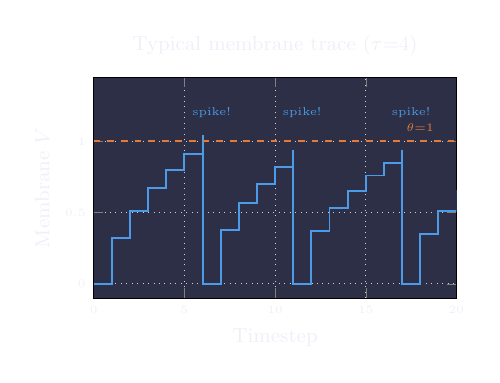
\begin{tikzpicture}[scale=0.82]
    \begin{axis}[
      width=7.2cm, height=5cm,
      xlabel={Timestep}, ylabel={Membrane $V$},
      xmin=0,xmax=20,ymin=-0.1,ymax=1.45,
      xtick={0,5,10,15,20},
      grid=major,grid style={dotted,gray!35},
      axis background/.style={fill=midbg},
      tick label style={color=lighttext,font=\tiny},
      label style={color=lighttext,font=\small},
      title style={color=lighttext,font=\small},
      title={Typical membrane trace ($\tau{=}4$)},
    ]
    \addplot[accent1,thick,const plot] coordinates {
      (0,0)(1,0.32)(2,0.51)(3,0.67)(4,0.80)(5,0.91)(6,1.04)
      (6.01,0)(7,0.38)(8,0.57)(9,0.70)(10,0.82)(11,0.93)
      (11.01,0)(12,0.37)(13,0.53)(14,0.65)(15,0.76)(16,0.85)
      (17,0.93)(17.01,0)(18,0.35)(19,0.51)(20,0.66)};
    \addplot[accent0,dashed,thick] coordinates {(0,1)(20,1)};
    \node[accent0,font=\tiny] at (axis cs:18,1.1) {$\theta{=}1$};
    \node[accent1,font=\tiny] at (axis cs:6.5,1.2) {spike!};
    \node[accent1,font=\tiny] at (axis cs:11.5,1.2) {spike!};
    \node[accent1,font=\tiny] at (axis cs:17.5,1.2) {spike!};
    \end{axis}
  \end{tikzpicture}
  \vspace{0.15em}
  \begin{tcolorbox}[mybox]
    \scriptsize
    Spike rate $\approx 5$–15\% per step in practice.\\
    95\%-sparse pruning: only 5\% of $W_\text{rec}$ non-zero.\\
    \textbf{Combined: $\ll1\%$ of multiplications needed.}
  \end{tcolorbox}
\end{column}
\end{columns}
\end{frame}

% ── SLIDE 4: TPSAPU Backbone ─────────────────────────────────────────────────
\begin{frame}[shrink=8]{\tpsapu{} Backbone: One Matrix, Many Timescales}
\begin{columns}[T]
\begin{column}{0.48\textwidth}
  \textbf{Core idea: shared topology, different $\tau$}
  \vspace{0.3em}
  \begin{enumerate}\small
    \item Input token $x_t$ projected: $\;z_t = W_\text{in}x_t$
    \item For each of $N_\tau$ reservoirs in parallel:\\
          $V^\tau_t \mathrel{+}= (z_t + W_\text{rec}s^\tau_{t-1} - V^\tau_t)/\tau$
    \item Spike: $s^\tau_t = \mathbf{1}[V^\tau_t \geq 1]$, reset $V^\tau_t \leftarrow 0$
    \item Output: $\text{cat}(V^{\tau_1}_t,\ldots,V^{\tau_N}_t)$ \textbf{per step}
  \end{enumerate}
  \vspace{0.4em}
  \begin{tcolorbox}[mybox,title=Parameter sharing]
    \scriptsize
    $W_\text{in} \in \mathbb{R}^{d\times d}$, $W_\text{rec} \in \mathbb{R}^{d\times d}$
    are \hl{shared} across all $N_\tau$ reservoirs.\\
    MNIST: $d{=}64$, $N_\tau{=}3$ $\Rightarrow$ 192 features/step.\\
    ImageNet: $d{=}64$, $N_\tau{=}8$ $\Rightarrow$ \hl{512 features/step}.
  \end{tcolorbox}
  \vspace{0.2em}
  \begin{tcolorbox}[mybox,title=Sparsity schedule]
    \scriptsize
    L2-driven magnitude pruning ramps from 0 to \hl{95\%} over 24 epochs.
    Final 6 epochs stabilize at the fixed mask.
    Only 5\% of recurrent weights remain non-zero.
  \end{tcolorbox}
\end{column}
\begin{column}{0.48\textwidth}
  \centering
  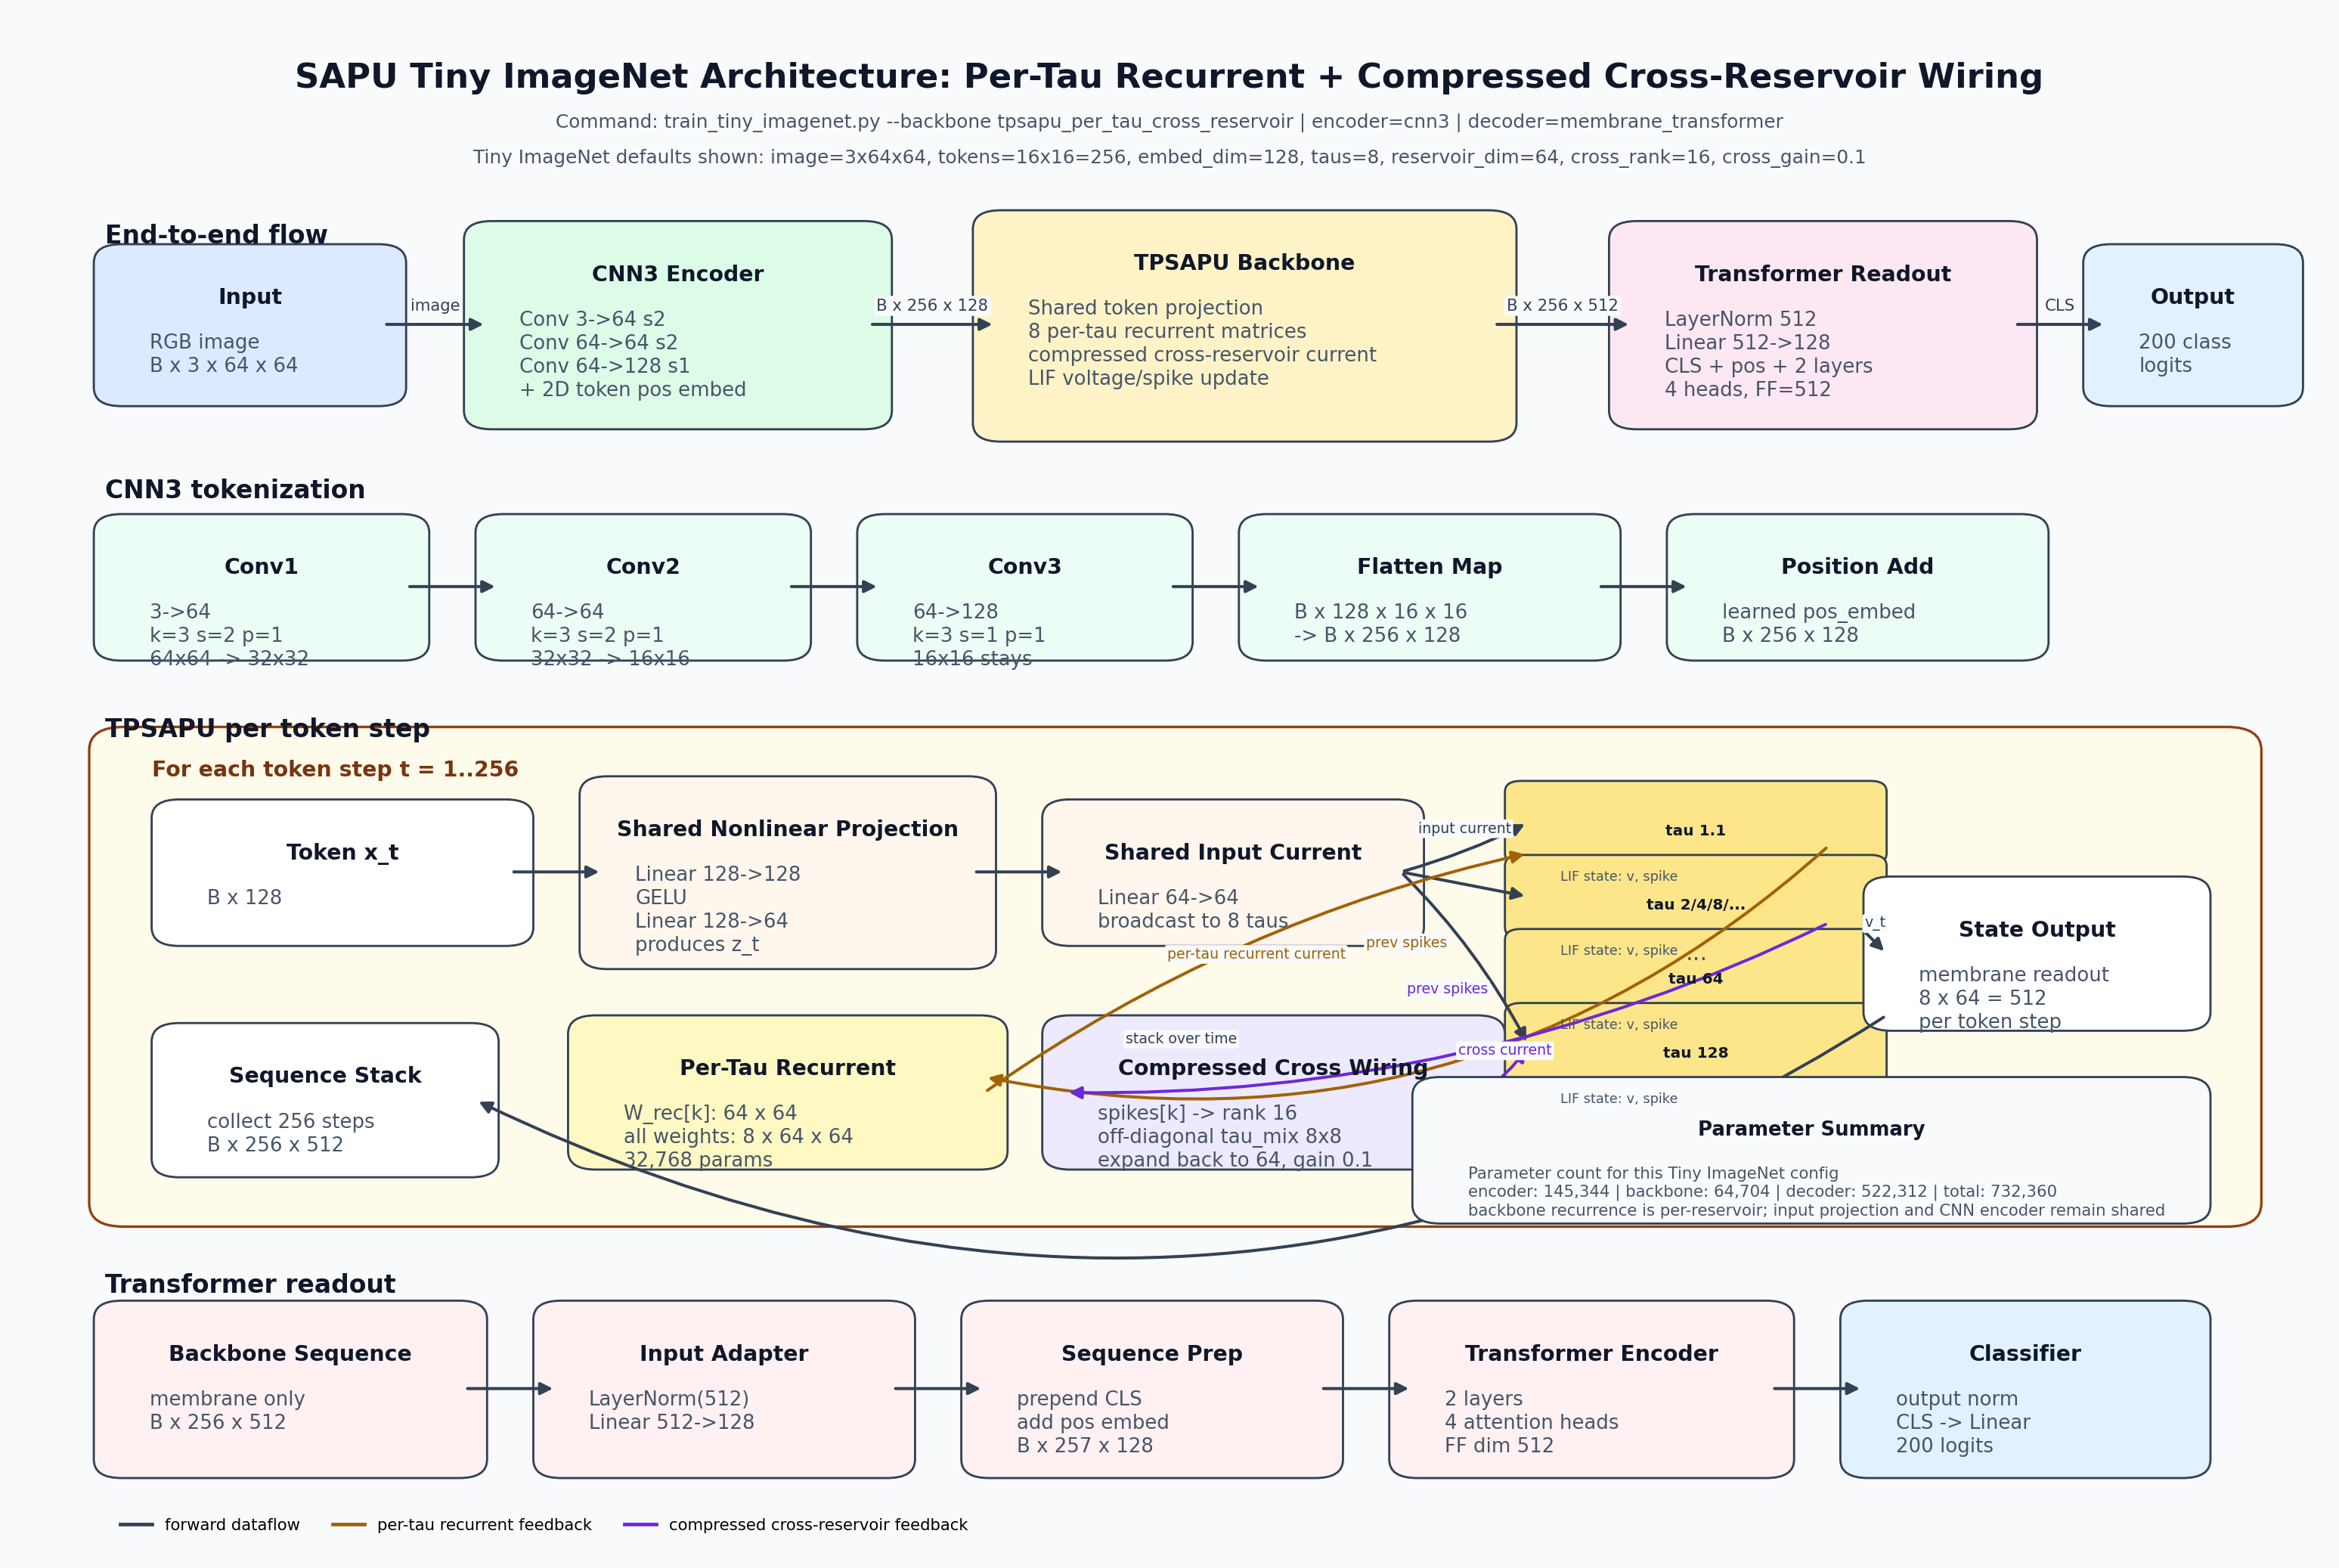
\includegraphics[width=\linewidth]{../visualizations/architecture/tpsapu_per_tau_cross_reservoir_architecture.png}
  {\scriptsize\color{subtletext} Overview of LLM versions of SAPU, both parallel and serial.}
\end{column}
\end{columns}
\end{frame}

% ── SLIDE 5: Full Pipeline ────────────────────────────────────────────────────
\begin{frame}[shrink=8]{End-to-End Pipeline: Encoder → Backbone → Decoder}
\begin{columns}[T]
\begin{column}{0.52\textwidth}
  \textbf{The three stages:}
  \vspace{0.3em}

  \begin{tcolorbox}[mybox,title={\orange{Encoder} — image $\to$ token sequence}]
    \scriptsize
    \texttt{cnn3}: Conv(s=2)$\to$Conv(s=2)$\to$Conv(s=1)\\
    On 64$\times$64: $(B,3,64,64)\to(B,256,128)$ — \hl{256 tokens, 16$\times$16 grid}\\
    \texttt{res\_cnn}: same + residual, concatenate both layers $\to$ 512 tokens
  \end{tcolorbox}
  \vspace{0.3em}
  \begin{tcolorbox}[mybox,title={\blue{Backbone} — tokens $\to$ reservoir states}]
    \scriptsize
    Each token is one LIF step for all $N_\tau$ reservoirs in parallel.\\
    Output (membrane, `\texttt{pooling=none}`):
    $(B, 256, N_\tau \cdot d_\text{res})$, e.g.\ $(B,256,512)$
  \end{tcolorbox}
  \vspace{0.3em}
  \begin{tcolorbox}[mybox,title={\green{Decoder} — states $\to$ logits}]
    \scriptsize
    \textbf{MLP variants:} pool last/mean, classify\\
    \textbf{Transformer:} LayerNorm+Linear$\to$CLS+256 positions$\to$2-layer encoder$\to$classify\\
    model\_dim=128, 4 heads, 512-FFN, \textbf{bidirectional}, pooling=none
  \end{tcolorbox}
\end{column}
\begin{column}{0.44\textwidth}
  \vspace{0.5em}
  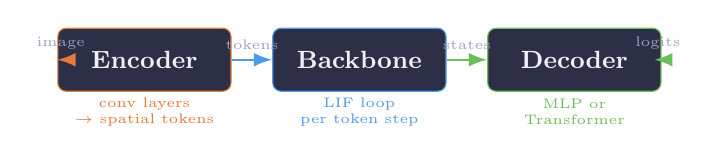
\begin{tikzpicture}[scale=0.78,every node/.style={font=\small}]
    \node[draw=accent0,fill=midbg,rounded corners=3pt,
          minimum width=2.2cm,minimum height=0.8cm,text=lighttext]
      (enc) at (0,0) {\textbf{Encoder}};
    \node[draw=accent1,fill=midbg,rounded corners=3pt,
          minimum width=2.2cm,minimum height=0.8cm,text=lighttext]
      (bb) at (3.5,0) {\textbf{Backbone}};
    \node[draw=accent2,fill=midbg,rounded corners=3pt,
          minimum width=2.2cm,minimum height=0.8cm,text=lighttext]
      (dec) at (7,0) {\textbf{Decoder}};
    \draw[-{Latex},thick,accent0] (-1.3,0)--(enc)
      node[midway,above,font=\tiny,color=subtletext]{image};
    \draw[-{Latex},thick,accent1] (enc)--(bb)
      node[midway,above,font=\tiny,color=subtletext]{tokens};
    \draw[-{Latex},thick,accent2] (bb)--(dec)
      node[midway,above,font=\tiny,color=subtletext]{states};
    \draw[-{Latex},thick,accent2] (dec)--(8.3,0)
      node[midway,above,font=\tiny,color=subtletext]{logits};
    \node[color=accent0,font=\tiny,text width=2cm,align=center]
      at (0,-0.85) {conv layers\\$\to$ spatial tokens};
    \node[color=accent1,font=\tiny,text width=2cm,align=center]
      at (3.5,-0.85) {LIF loop\\per token step};
    \node[color=accent2,font=\tiny,text width=2cm,align=center]
      at (7,-0.85) {MLP or\\Transformer};
  \end{tikzpicture}
  \vspace{0.4em}
  \renewcommand{\arraystretch}{1.15}
  {\scriptsize
  \begin{tabular}{lrrr}
    \toprule
    & MNIST & TinyIM (sm) & TinyIM (lg) \\
    \midrule
    Image & 28$^2$ & 64$^2$ & 64$^2$ \\
    Tokens & 49 & \hl{256} & \hl{512} \\
    $N_\tau$ & 3 & 8 & 8 \\
    $d_\text{res}$ & 64 & 64 & 256 \\
    Neurons & 192 & 512 & \hl{2048} \\
    Params & $\sim$200k & 702k & 1.65M \\
    \bottomrule
  \end{tabular}}
\end{column}
\end{columns}
\end{frame}

% ── SLIDE 6: MNIST Sanity Check ──────────────────────────────────────────────
\begin{frame}[shrink=12]{MNIST Sanity Check: 42 Encoder$\times$Decoder Combinations}
\begin{columns}[T]
\begin{column}{0.50\textwidth}
  \vspace{-0.3em}
  {\tiny
  \renewcommand{\arraystretch}{1.0}
  \begin{tabular}{l|cccccc}
    \toprule
    \makecell{\textbf{Encoder}} &
    \rotatebox{55}{\texttt{linear}} &
    \rotatebox{55}{\texttt{mem\_mlp}} &
    \rotatebox{55}{\texttt{spike\_mlp}} &
    \rotatebox{55}{\texttt{both\_mlp}} &
    \rotatebox{55}{\texttt{all\_state}} &
    \rotatebox{55}{\texttt{lif\_count}} \\
    \midrule
    \texttt{cnn3}     & 99.4 & 99.3 & \orange{98.7} & \hl{99.4} & \hl{99.4} & 99.3 \\
    \texttt{res\_cnn} & 99.3 & 99.3 & \orange{98.7} & \hl{99.4} & \hl{99.4} & 99.1 \\
    \texttt{cnn2}     & 99.1 & 99.1 & \orange{96.9} & 99.2 & 99.2 & 99.0 \\
    \texttt{mlp\_pch} & 98.4 & 98.6 & \orange{84.9} & 98.6 & \hl{98.7} & 98.0 \\
    \texttt{rows}     & 97.0 & 98.3 & \orange{94.0} & 98.4 & 98.4 & 96.8 \\
    \texttt{lin\_pch} & 97.4 & 98.1 & \orange{90.1} & 97.9 & 98.3 & 97.0 \\
    \texttt{lif\_2x2} & 91.3 & 93.4 & \orange{61.7} & 92.6 & 95.1 & 90.2 \\
    \bottomrule
  \end{tabular}}
  \vspace{0.3em}
  \begin{tcolorbox}[mybox]
    \scriptsize
    Best: \hl{99.41\%} (cnn3 + both\_mlp or all\_state\_mlp).\\
    \orange{spike\_mlp always worst} — raw binary outputs too noisy.\\
    20 epochs, no pruning, ${\sim}200$k params.
  \end{tcolorbox}
\end{column}
\begin{column}{0.46\textwidth}
  \textbf{Observations:}
  \begin{itemize}\scriptsize
    \item \hl{Encoder quality dominates}: CNN $>$ patch $>$ rows
    \item lif\_2x2 severely limited — biologically motivated
          but 196 weak binary tokens hurt
    \item Combining membrane + spike (\texttt{both\_mlp}) \hl{always beats single modality}
    \item Even a linear decoder over TPSAPU membranes achieves $>$97\%
    \item Architecture is robust — 35 of 42 combinations exceed 96\%
  \end{itemize}
  \vspace{0.2em}
  \begin{block}{Sanity check passed}
    \scriptsize TPSAPU matches or approaches standard CNN baselines on MNIST
    with far fewer parameters and binary activations.
  \end{block}
\end{column}
\end{columns}
\end{frame}

% ── SLIDE 7: What Neurons See (MNIST) ────────────────────────────────────────
\begin{frame}[shrink=5]{What the Reservoir Sees: Tokens \& Voltage Matrix}
\begin{columns}[T]
\begin{column}{0.50\textwidth}
  \centering
  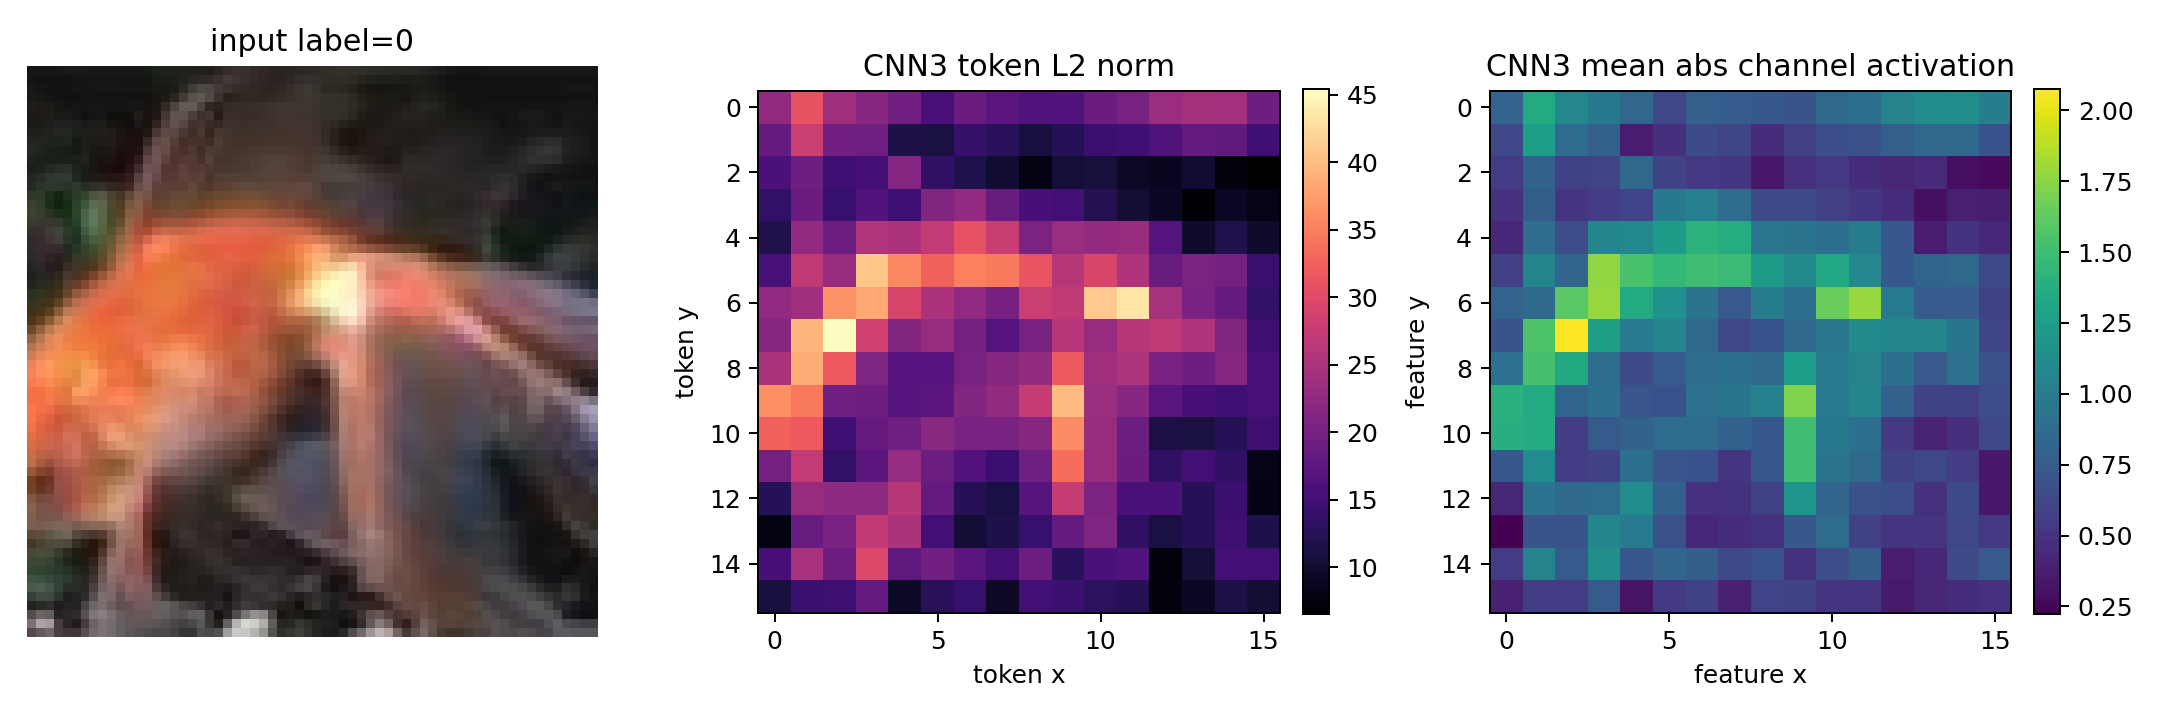
\includegraphics[width=\linewidth]{../visualizations/cnn3_voltages/validation_0/input_and_cnn3_tokens.png}
  {\scriptsize\color{subtletext}
    Left: input\quad Centre: token L2-norm heatmap\quad Right: channel activations}
  \vspace{0.3em}
  \begin{itemize}\scriptsize
    \item CNN concentrates high-norm tokens on \hl{object edges}
    \item Background patches $\approx$ zero norm — sparse input
    \item The backbone sees this as a \textbf{sequence of timesteps}
  \end{itemize}
\end{column}
\begin{column}{0.46\textwidth}
  \centering
  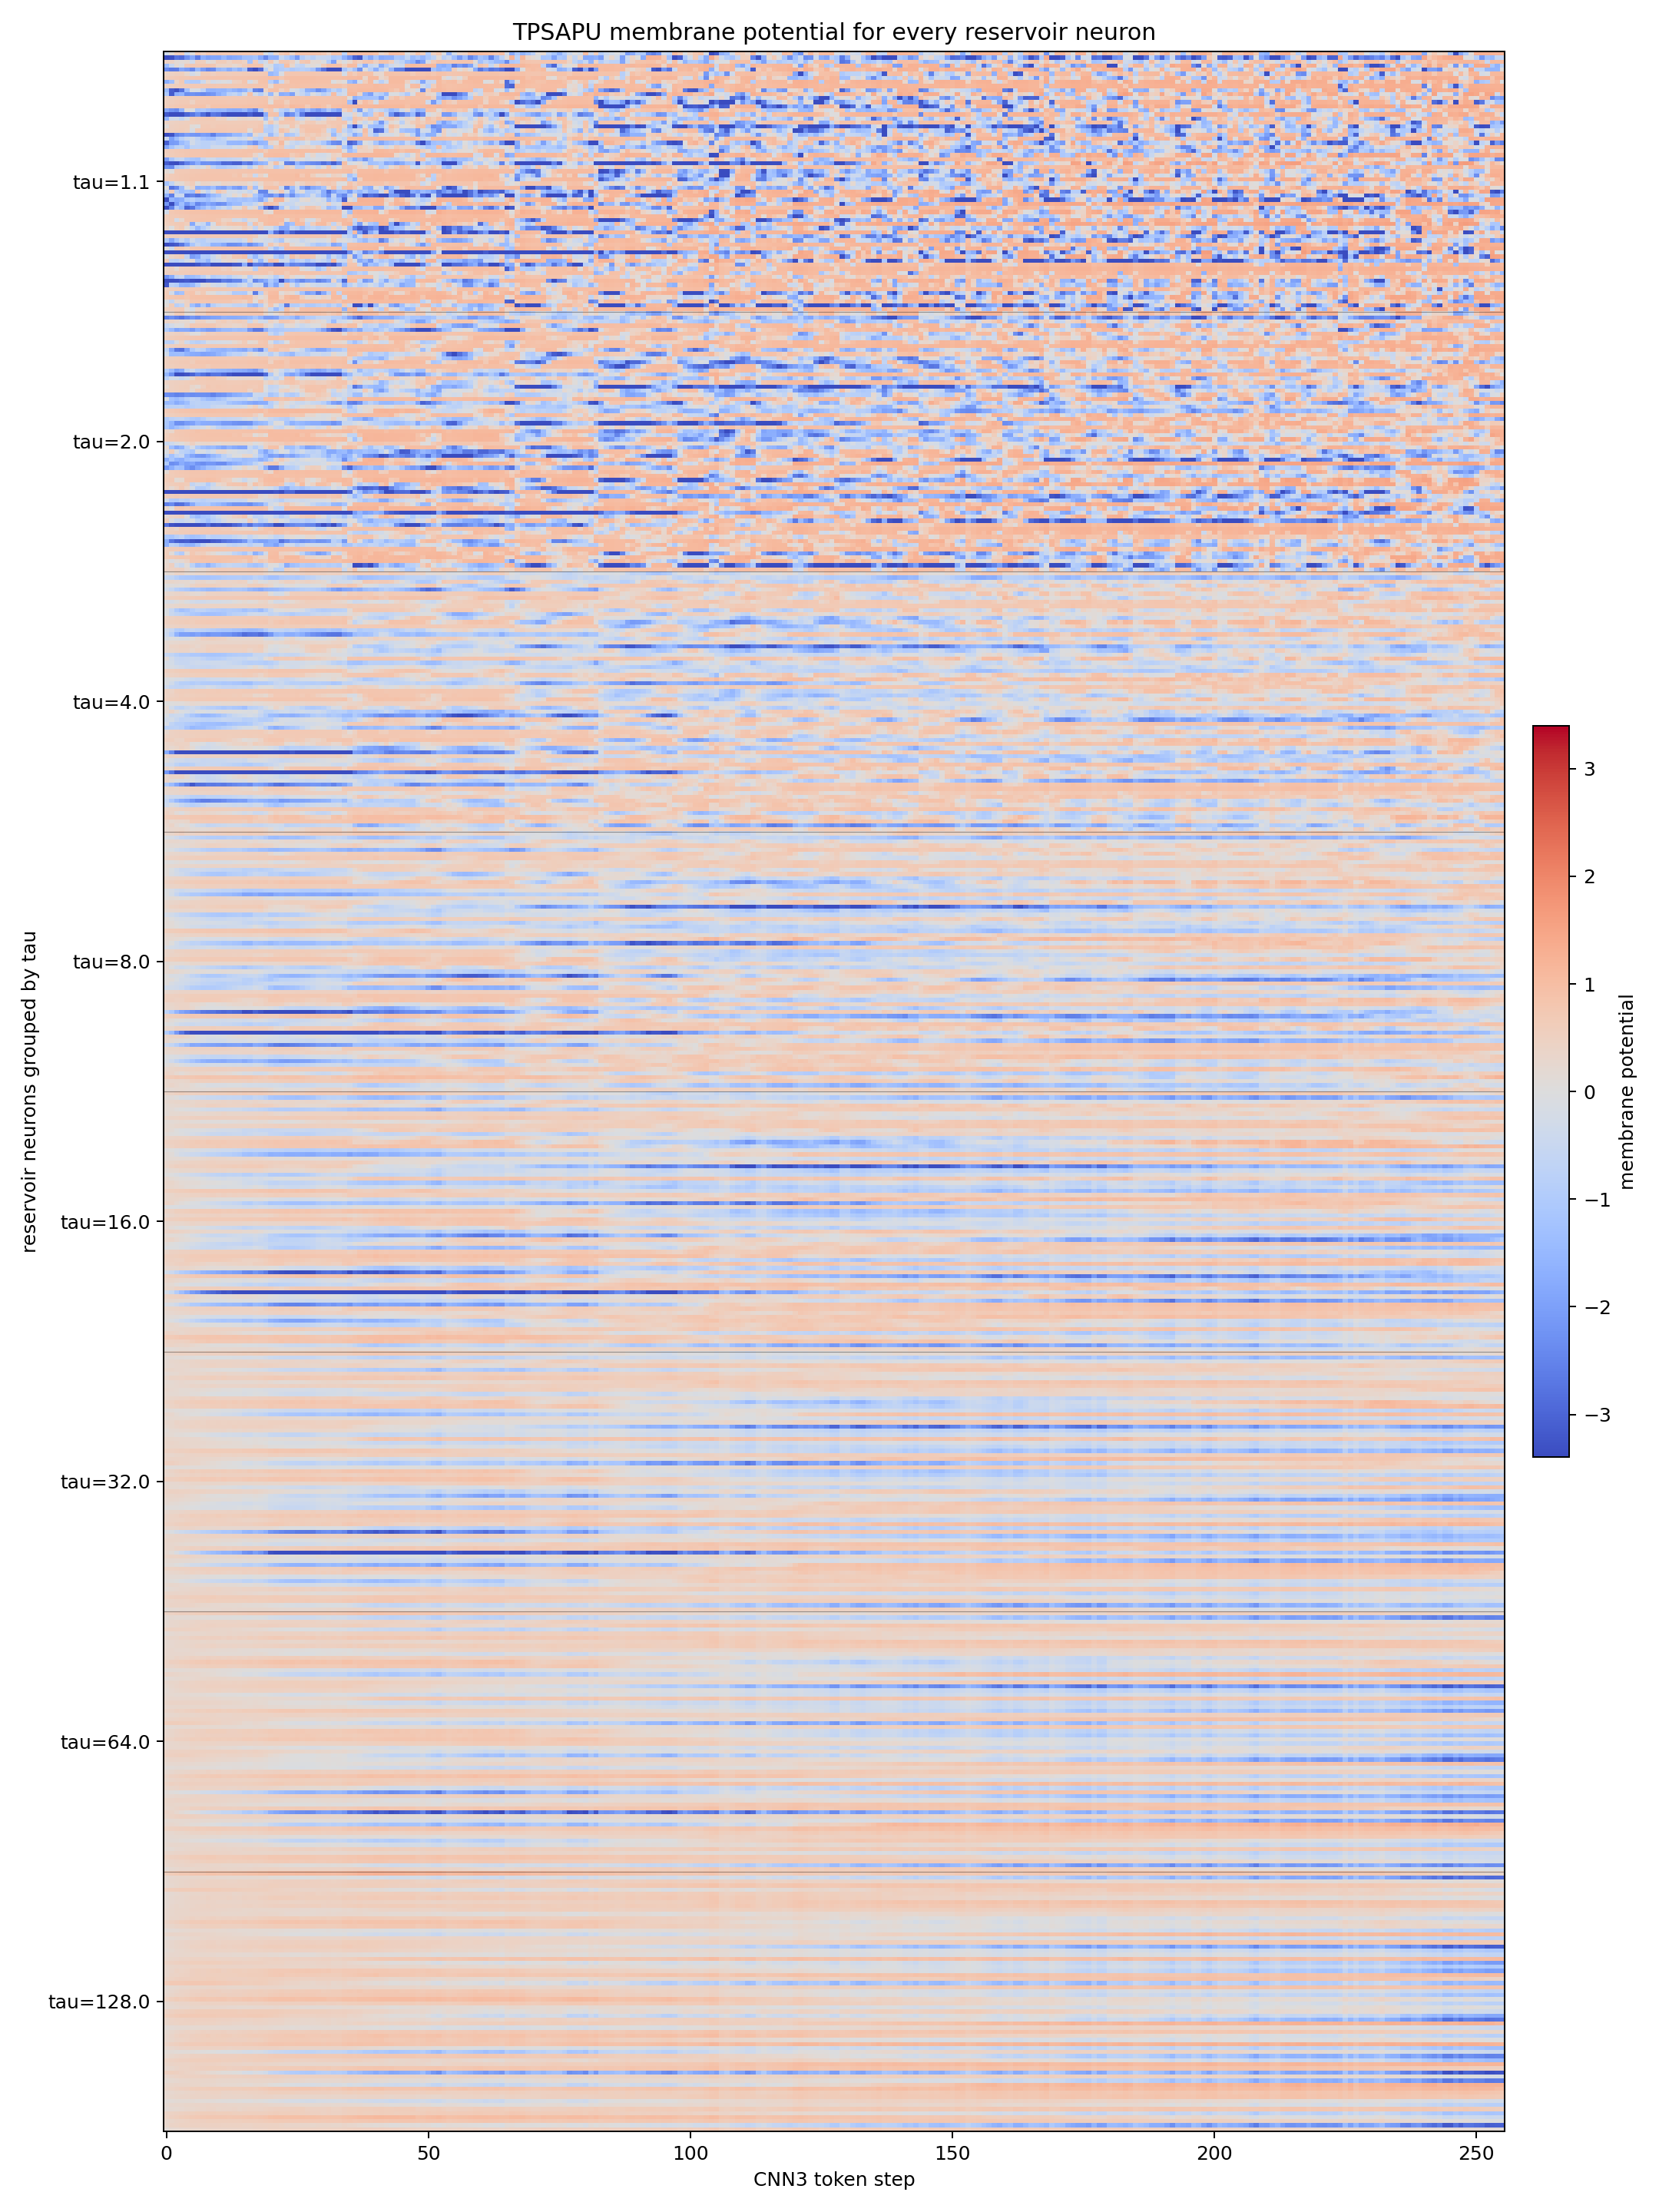
\includegraphics[width=\linewidth]{../visualizations/cnn3_voltages/validation_0/tpsapu_all_neuron_voltage_matrix.png}
  {\scriptsize\color{subtletext}
    Rows = neurons grouped by $\tau$. Cols = token steps. Coolwarm scale.}
  \vspace{0.3em}
  \begin{itemize}\scriptsize
    \item Fast $\tau$ reservoirs (top rows): sharp reactions, rapid reset
    \item Slow $\tau$ reservoirs (bottom rows): smooth integration
    \item Most neurons \hl{never fire} at a given step ($>$90\% zeros)
  \end{itemize}
\end{column}
\end{columns}
\end{frame}

% ── SLIDE 8: Temporal Dynamics ────────────────────────────────────────────────
\begin{frame}[shrink=15]{Temporal Dynamics: Per-$\tau$ Traces \& Spike Heatmaps}
\begin{columns}[T]
\begin{column}{0.50\textwidth}
  \centering
  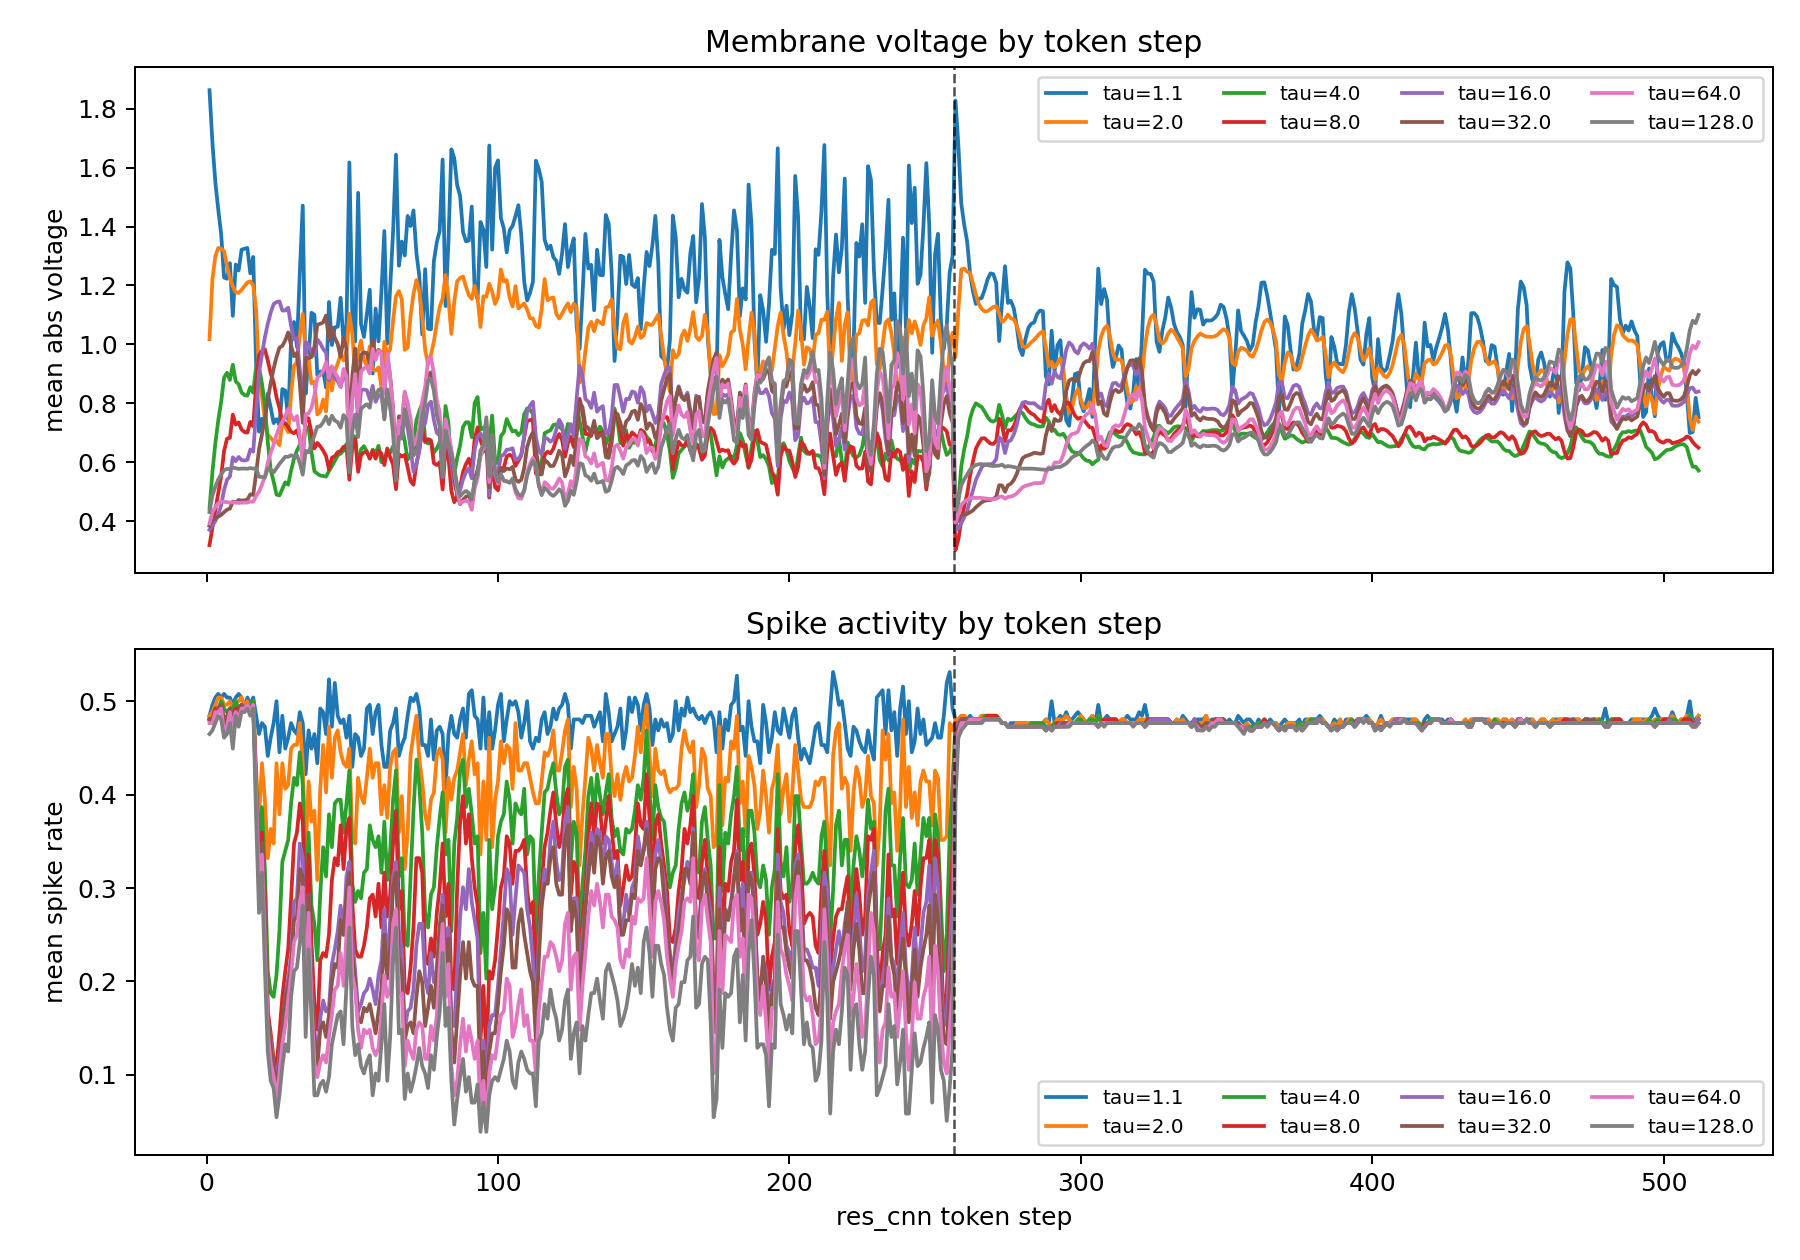
\includegraphics[width=\linewidth]{../visualizations/res_cnn_cross_both_transformer_best/validation_0/tpsapu_tau_traces.png}
  {\scriptsize\color{subtletext}
    Mean membrane voltage (solid) and spike rate (dashed) per $\tau$, over token steps.}
\end{column}
\begin{column}{0.46\textwidth}
  \centering
  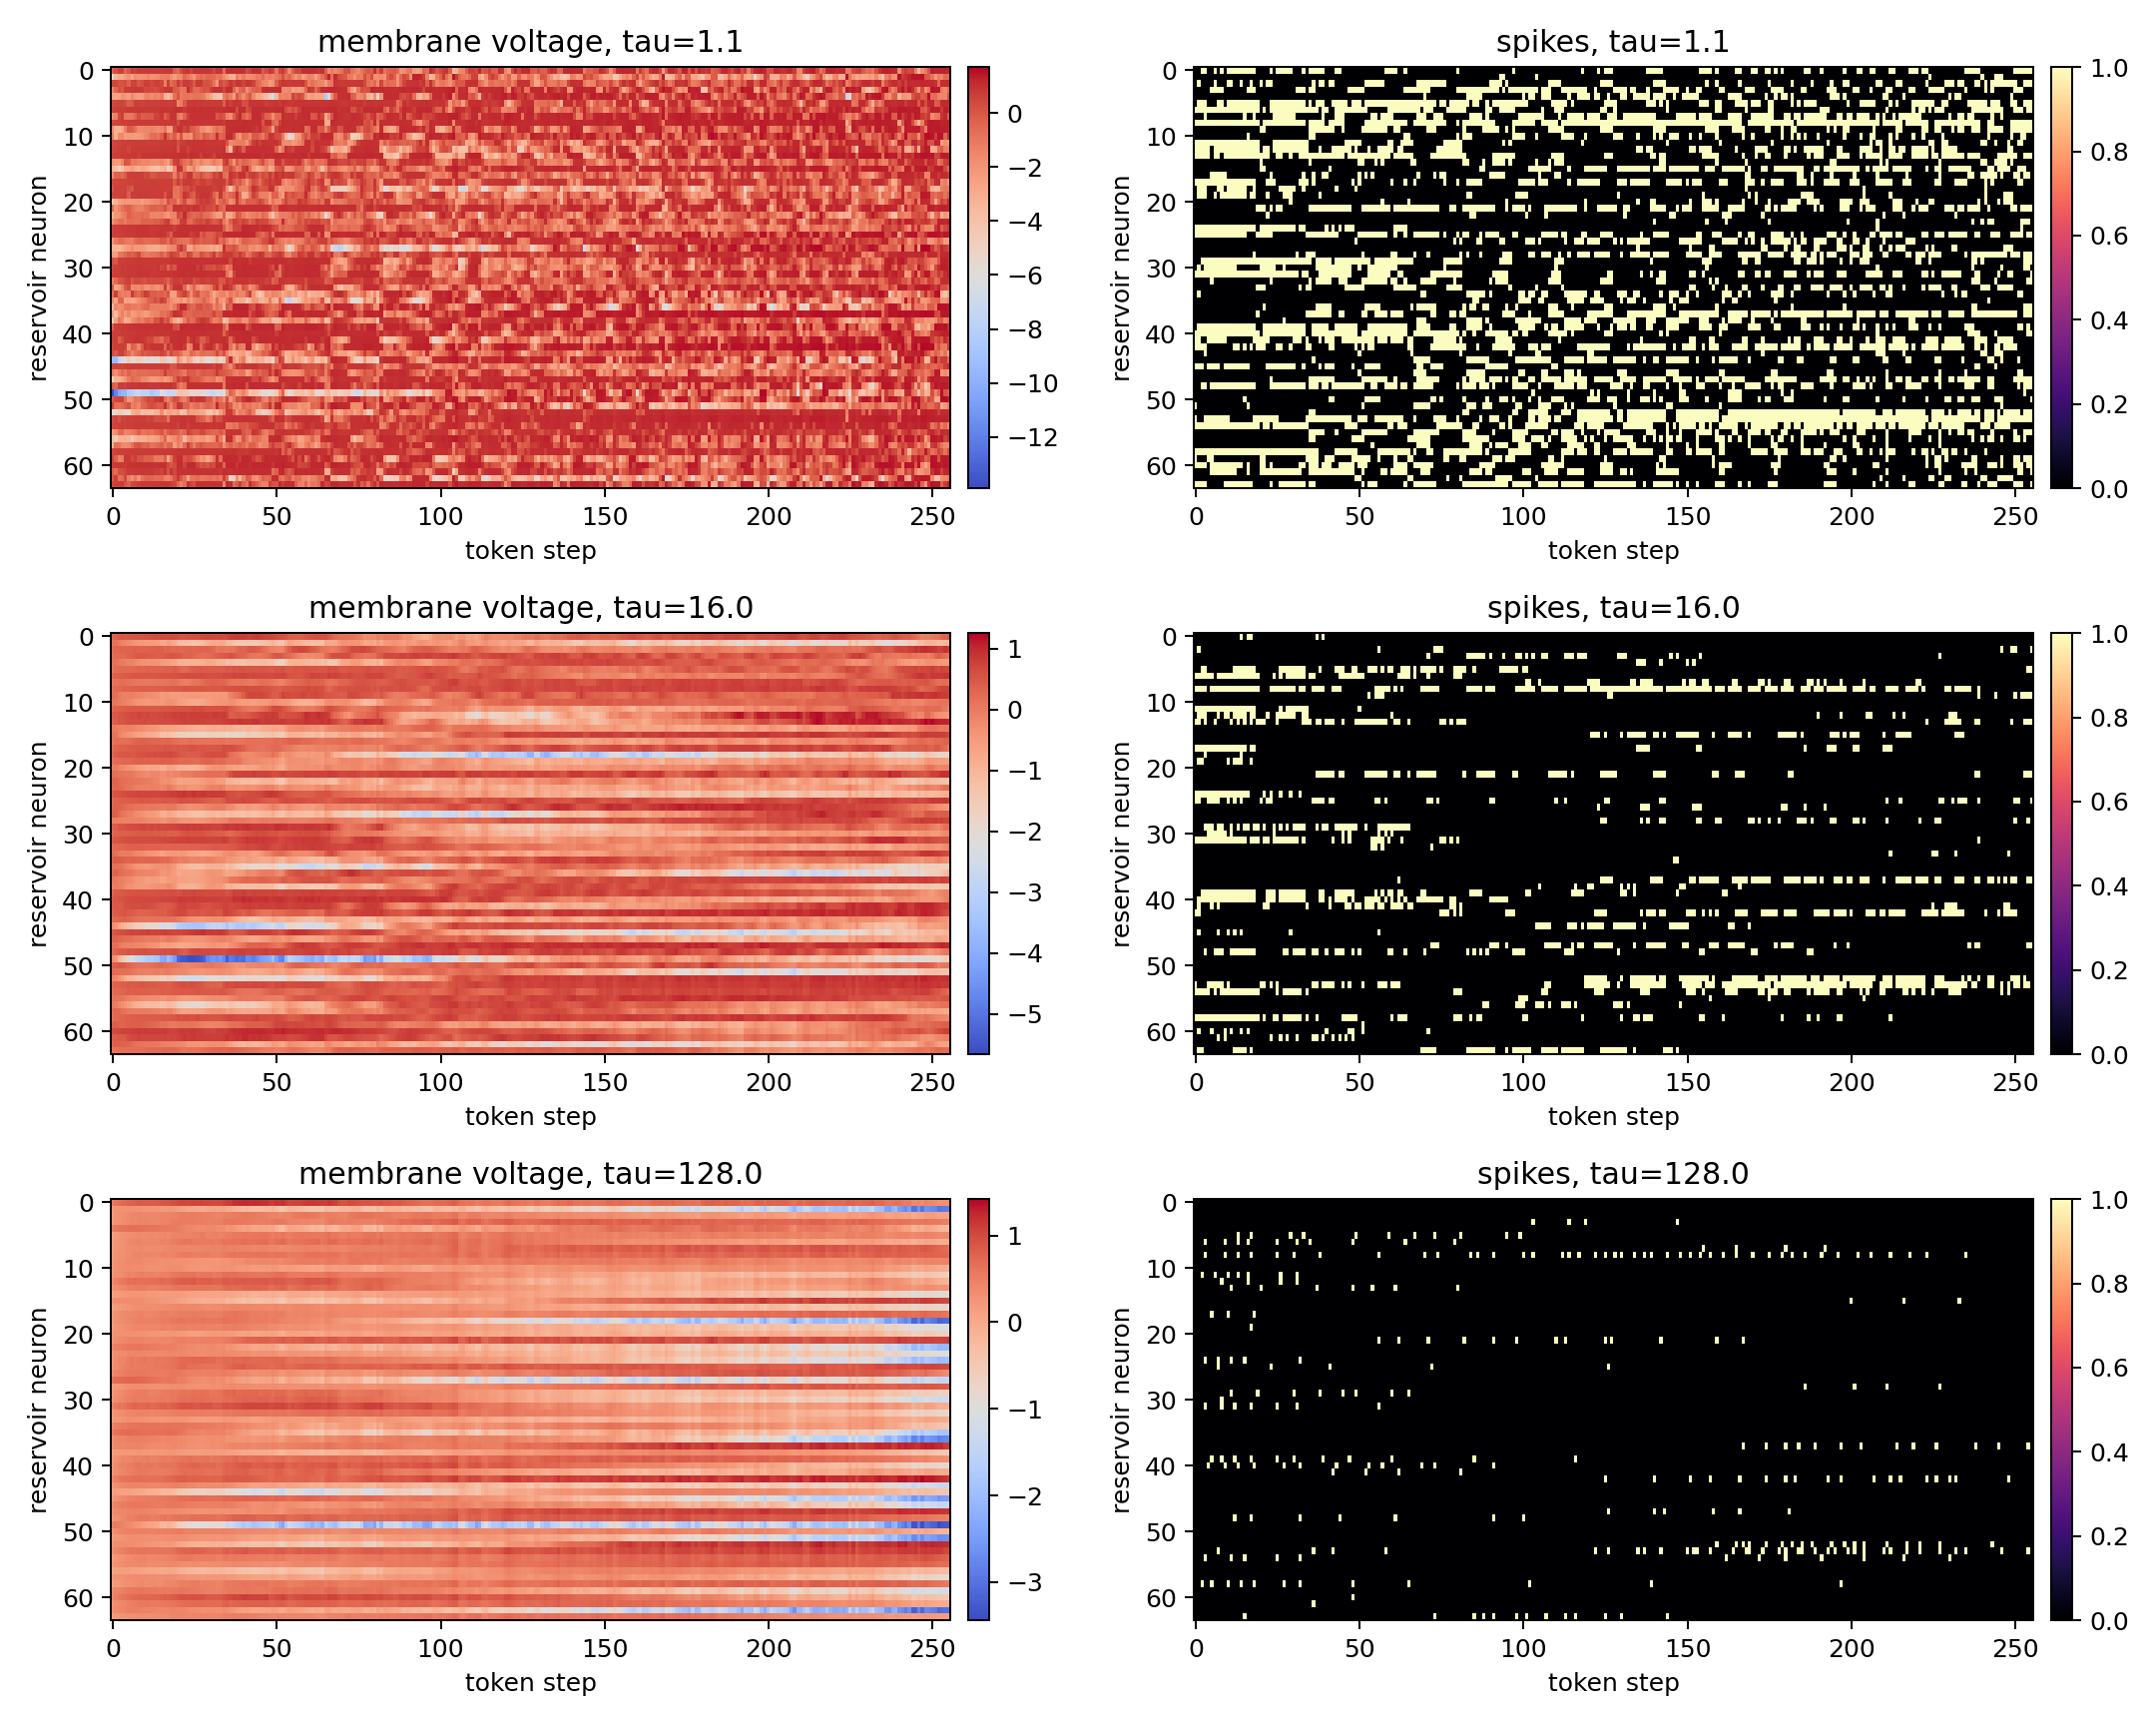
\includegraphics[width=\linewidth]{../visualizations/cnn3_voltages/validation_0/tpsapu_neuron_heatmaps.png}
  {\scriptsize\color{subtletext}
    Per-neuron membrane (left) and spikes (right) for selected $\tau$ values.}
\end{column}
\end{columns}
\vspace{0.3em}
\begin{tcolorbox}[mybox]
  \scriptsize
  \textbf{Multi-timescale hypothesis:} fast reservoirs ($\tau\approx1.1$) react sharply to edges and local features.
  Slow reservoirs ($\tau{=}128$) build a global summary over the whole sequence.
  The decoder sees \emph{all} $\tau$-bands simultaneously — a richer feature than any single timescale.
  This is what differentiates \tpsapu{} from a single-state RNN: \hl{multiple temporal abstractions at no extra recurrent cost}.
\end{tcolorbox}
\end{frame}

\begin{frame}[shrink=6]{MNIST: Spiking Rates \& Spectral Diagnostics}

\begin{columns}[T,onlytextwidth]
\begin{column}{0.57\textwidth}
  \centering
  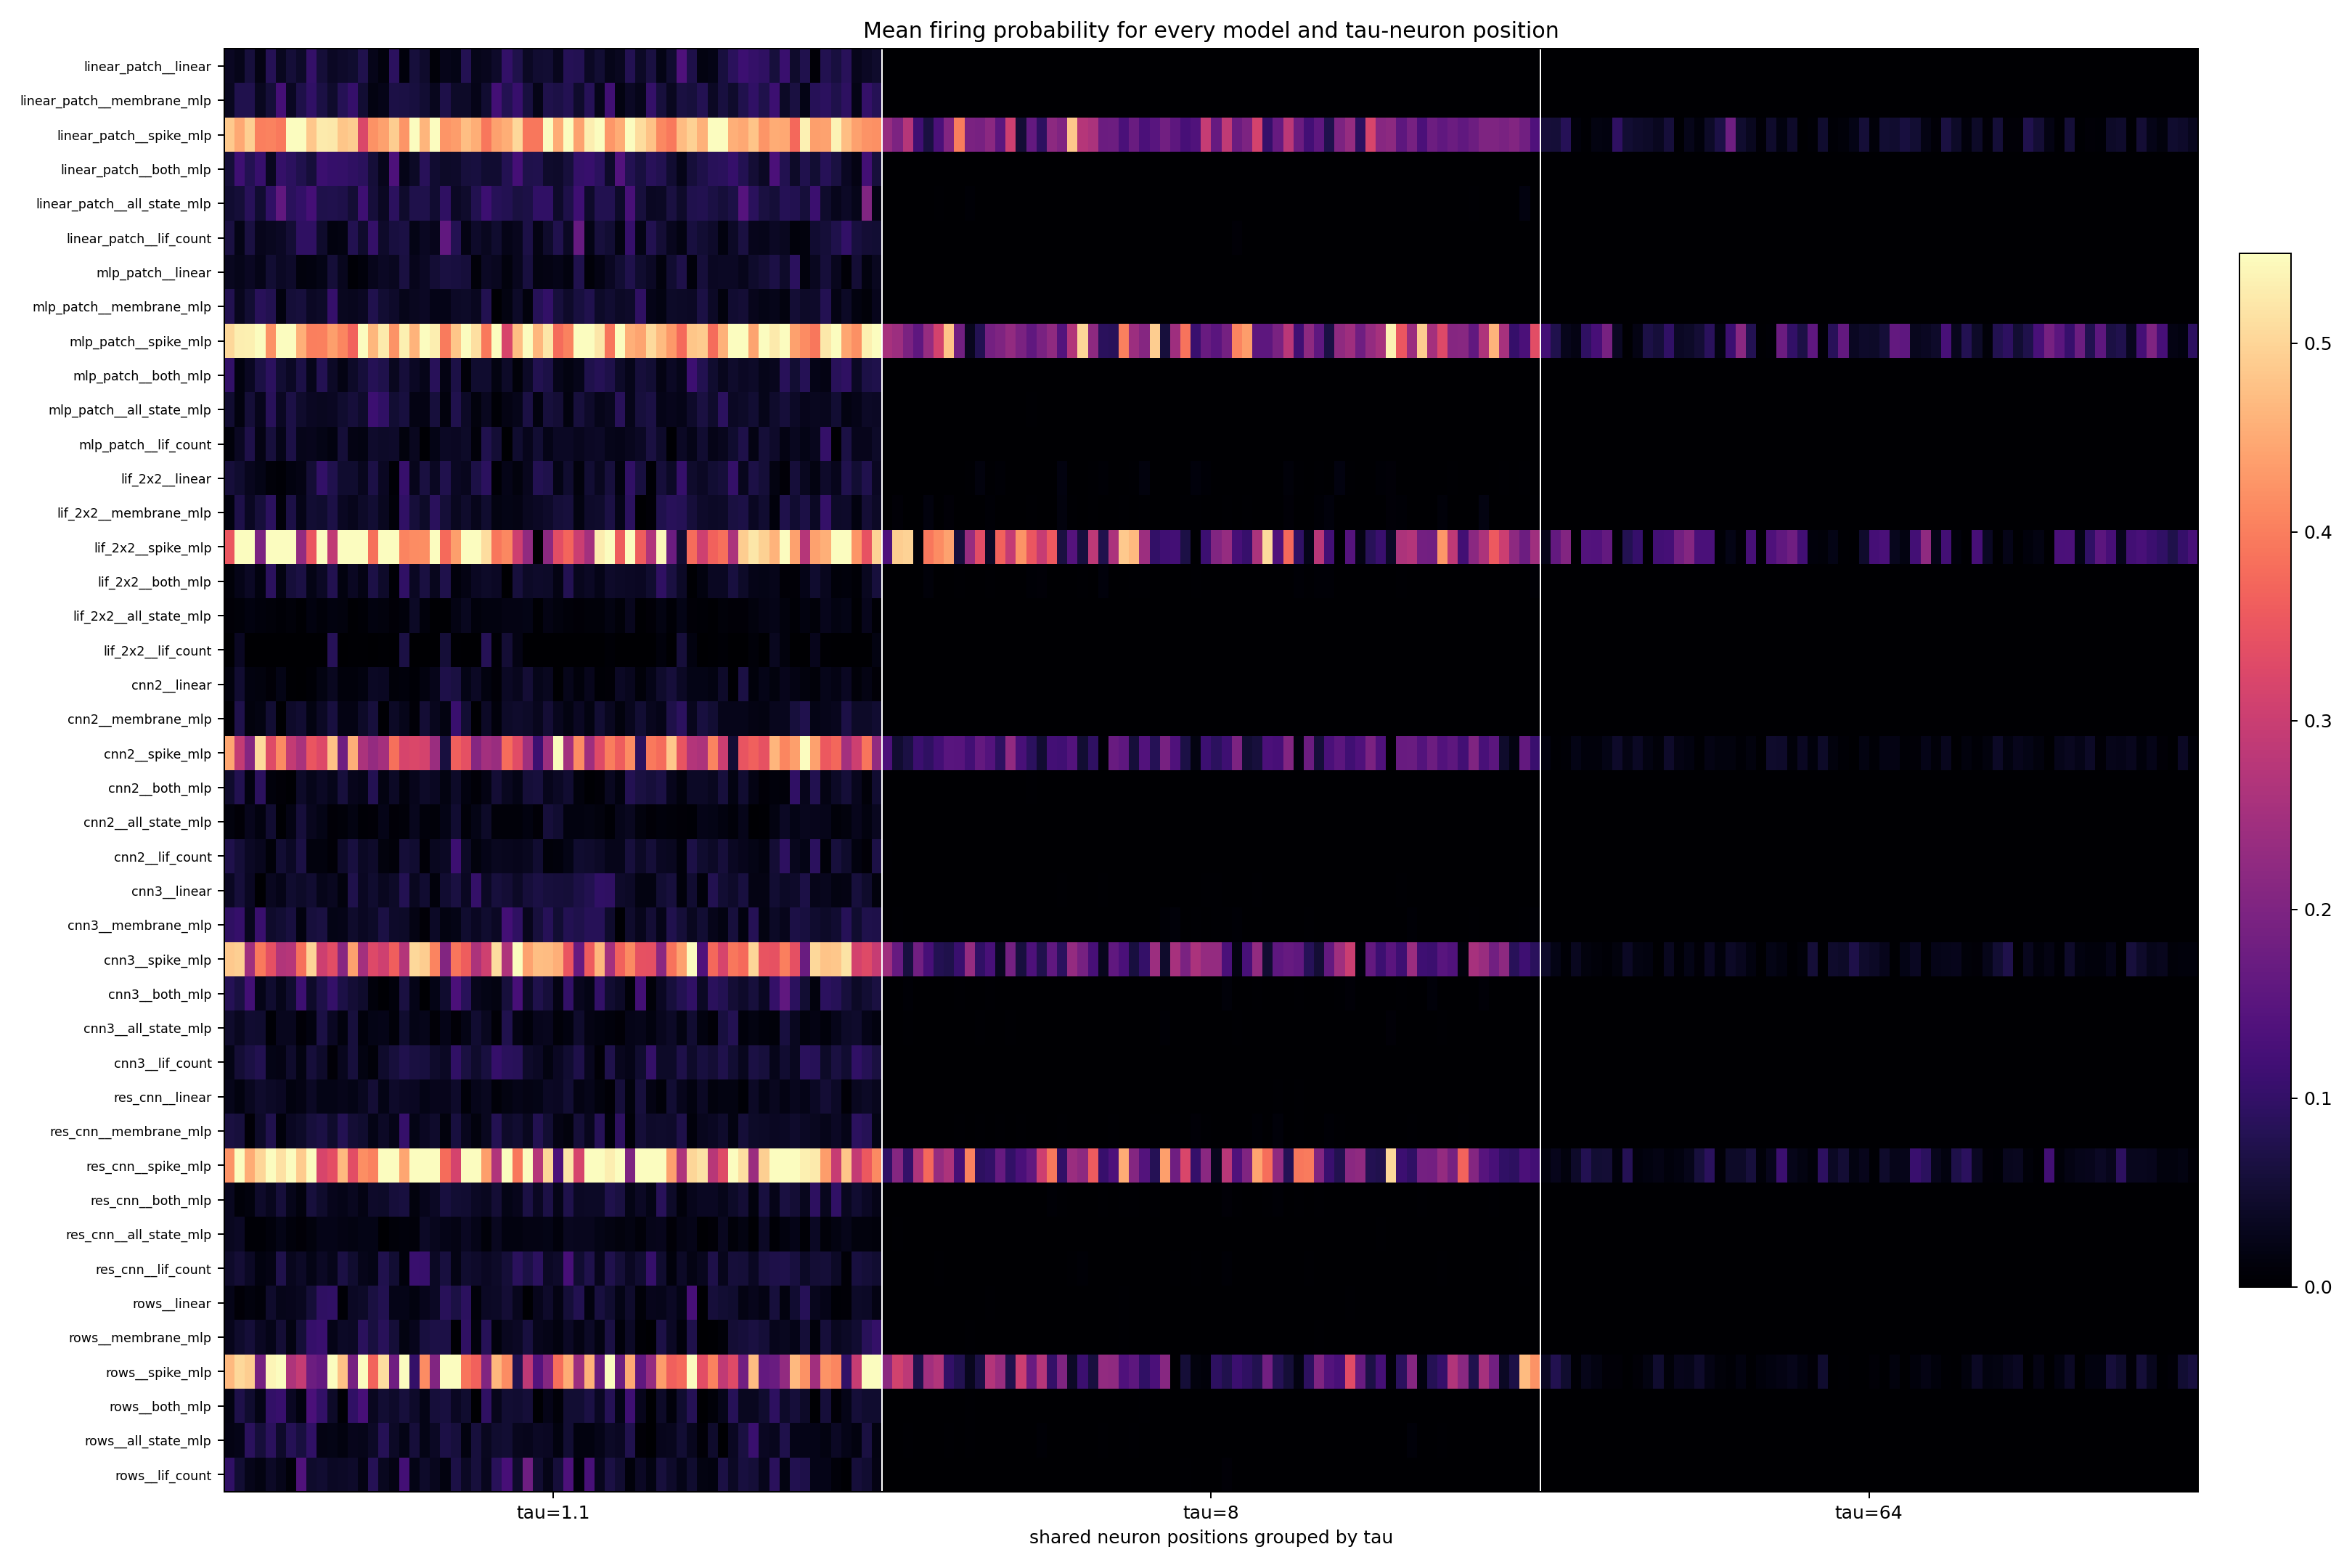
\includegraphics[
    width=\linewidth,
    height=0.76\textheight,
    keepaspectratio
  ]{../visualizations/mnist_sweep_spiking_topology/all_models_neuron_firing_rates.png}

  {\scriptsize\color{subtletext}
  Spike-only models learn to make neurons fire, but membrane readout still wins because voltage keeps weak evidence before a spike happens.}
\end{column}

\begin{column}{0.41\textwidth}
  \centering
  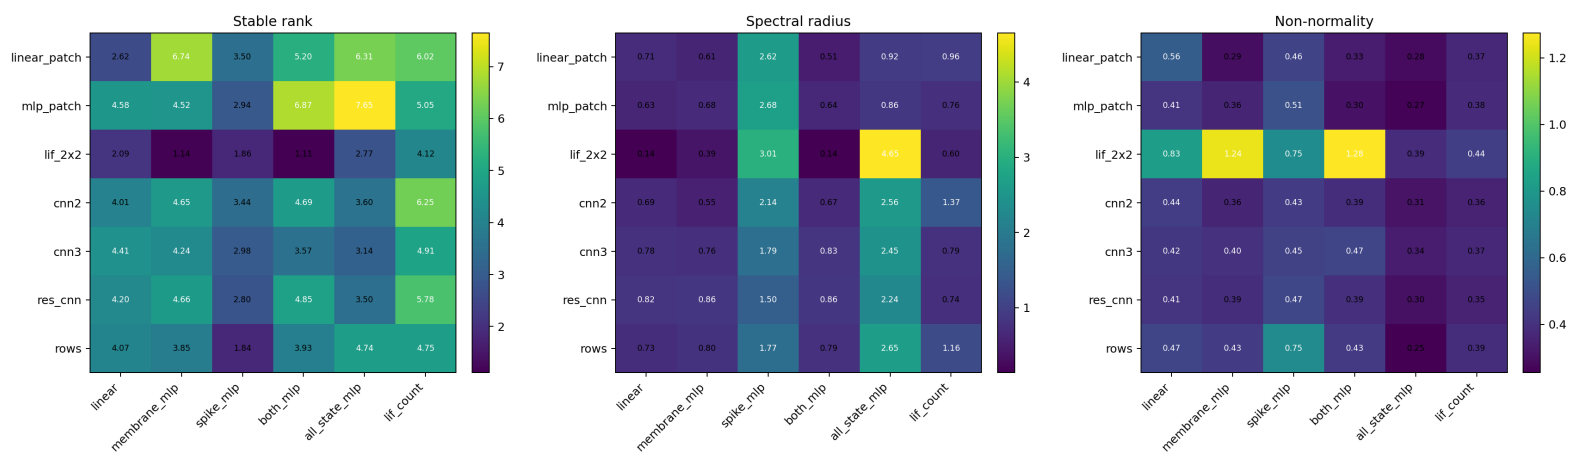
\includegraphics[
    width=\linewidth,
    height=0.39\textheight,
    keepaspectratio
  ]{../visualizations/mnist_sweep_checkpoint_analysis/weight_analysis_mnist.png}

  \vspace{0.4em}

  \begin{tcolorbox}[mybox]
  \scriptsize
  \textbf{How to read the spectrum plots:}

  \textbf{Stable rank} says how many independent directions the weights really use. Higher means the model is not relying on one dominant shortcut.

  \textbf{Spectral radius} says how strongly recurrent activity can be amplified. Too small forgets quickly; too large can become unstable or overly reactive.

  \textbf{Non-normality} means weights can temporarily amplify signals even if they look stable from eigenvalues alone. In ML terms: the dynamics may create short bursts of useful activity, but can also become harder to decode.
  \end{tcolorbox}
\end{column}
\end{columns}

\end{frame}

% ── SLIDE 9: MNIST Analysis ───────────────────────────────────────────────────
\begin{frame}[shrink=5]{MNIST Analysis: Insights \& Gaps}
\begin{columns}[T]
\begin{column}{0.48\textwidth}
  \begin{block}{What drives performance}
    \begin{enumerate}\small
      \item \textbf{Encoder quality} — CNNs beat patch, patch beats rows
      \item \textbf{Combined readout} — both/all-state beats single modality
      \item \textbf{Timescale diversity} — 3 taus better than 1
      \item \textbf{Recurrent dropout} — prevents shortcut paths
    \end{enumerate}
  \end{block}
  \vspace{0.3em}
  \begin{alertblock}{What doesn't help}
    \begin{itemize}\small
      \item Spike-only decoders — too noisy for classification
      \item lif\_2x2 encoder — strong biological motivation, poor results
      \item Larger reservoirs on MNIST ($d_\text{res}=64$ is sufficient)
    \end{itemize}
  \end{alertblock}
\end{column}
\begin{column}{0.48\textwidth}
  \begin{alertblock}{Missing experiments}
    \begin{itemize}\small
      \item Transformer decoders on MNIST — folder empty! Would likely push $>$99.5\%
      \item No pruning applied ($\texttt{prune\_epochs}=0$) — does 95\% sparsity hold on MNIST?
      \item No tau ablation — how much do you lose with $N_\tau=1$?
      \item No backbone-free baseline
      \item No comparison to SNNTorch
    \end{itemize}
  \end{alertblock}
  \vspace{0.3em}
  \begin{tcolorbox}[mybox]
    \scriptsize
    \textbf{Verdict:} TPSAPU achieves competitive MNIST accuracy ($99.4\%$) at $\sim200$k params with sparse binary processing.
    The core architecture is \hl{validated}.
    Scaling behaviour on harder tasks is the open question.
  \end{tcolorbox}
\end{column}
\end{columns}
\end{frame}

% ── SLIDE 10: CNN3 Encoder Deep Dive ─────────────────────────────────────────
\begin{frame}[shrink=5]{CNN3 Encoder: How the Image Becomes a Token Sequence}
\begin{columns}[T]
\begin{column}{0.50\textwidth}
  \textbf{Three convolutions, then flatten:}
  \vspace{0.3em}
  {\scriptsize
  \begin{tabular}{lll}
    \toprule
    Layer & Output shape & Covers \\
    \midrule
    Input & $(B,3,64,64)$ & full image \\
    Conv1 (s=2) & $(B,64,32,32)$ & 2$\times$2 px \\
    Conv2 (s=2) & $(B,64,16,16)$ & 4$\times$4 px \\
    Conv3 (s=1) & $(B,128,16,16)$ & 4$\times$4 px \\
    flatten+pos & $(B,\mathbf{256},128)$ & \hl{16$\times$16 grid} \\
    \bottomrule
  \end{tabular}}
  \vspace{0.4em}
  \begin{itemize}\small
    \item 256 tokens — each covers a \hl{4$\times$4 pixel block}
    \item Learnable positional embedding ($\sigma=0.02$)
    \item \texttt{patch\_size=8} in args is \textbf{ignored} by CNN encoders —
          grid size comes from convolution strides only
    \item GELU activations, light Dropout2d$(0.05)$
  \end{itemize}
  \vspace{0.3em}
  \begin{tcolorbox}[mybox]
    \scriptsize
    The TPSAPU backbone then processes the 256 tokens \textbf{one step at a time},
    treating the spatial raster-scan order as a temporal sequence.
  \end{tcolorbox}
\end{column}
\begin{column}{0.46\textwidth}
  \centering
  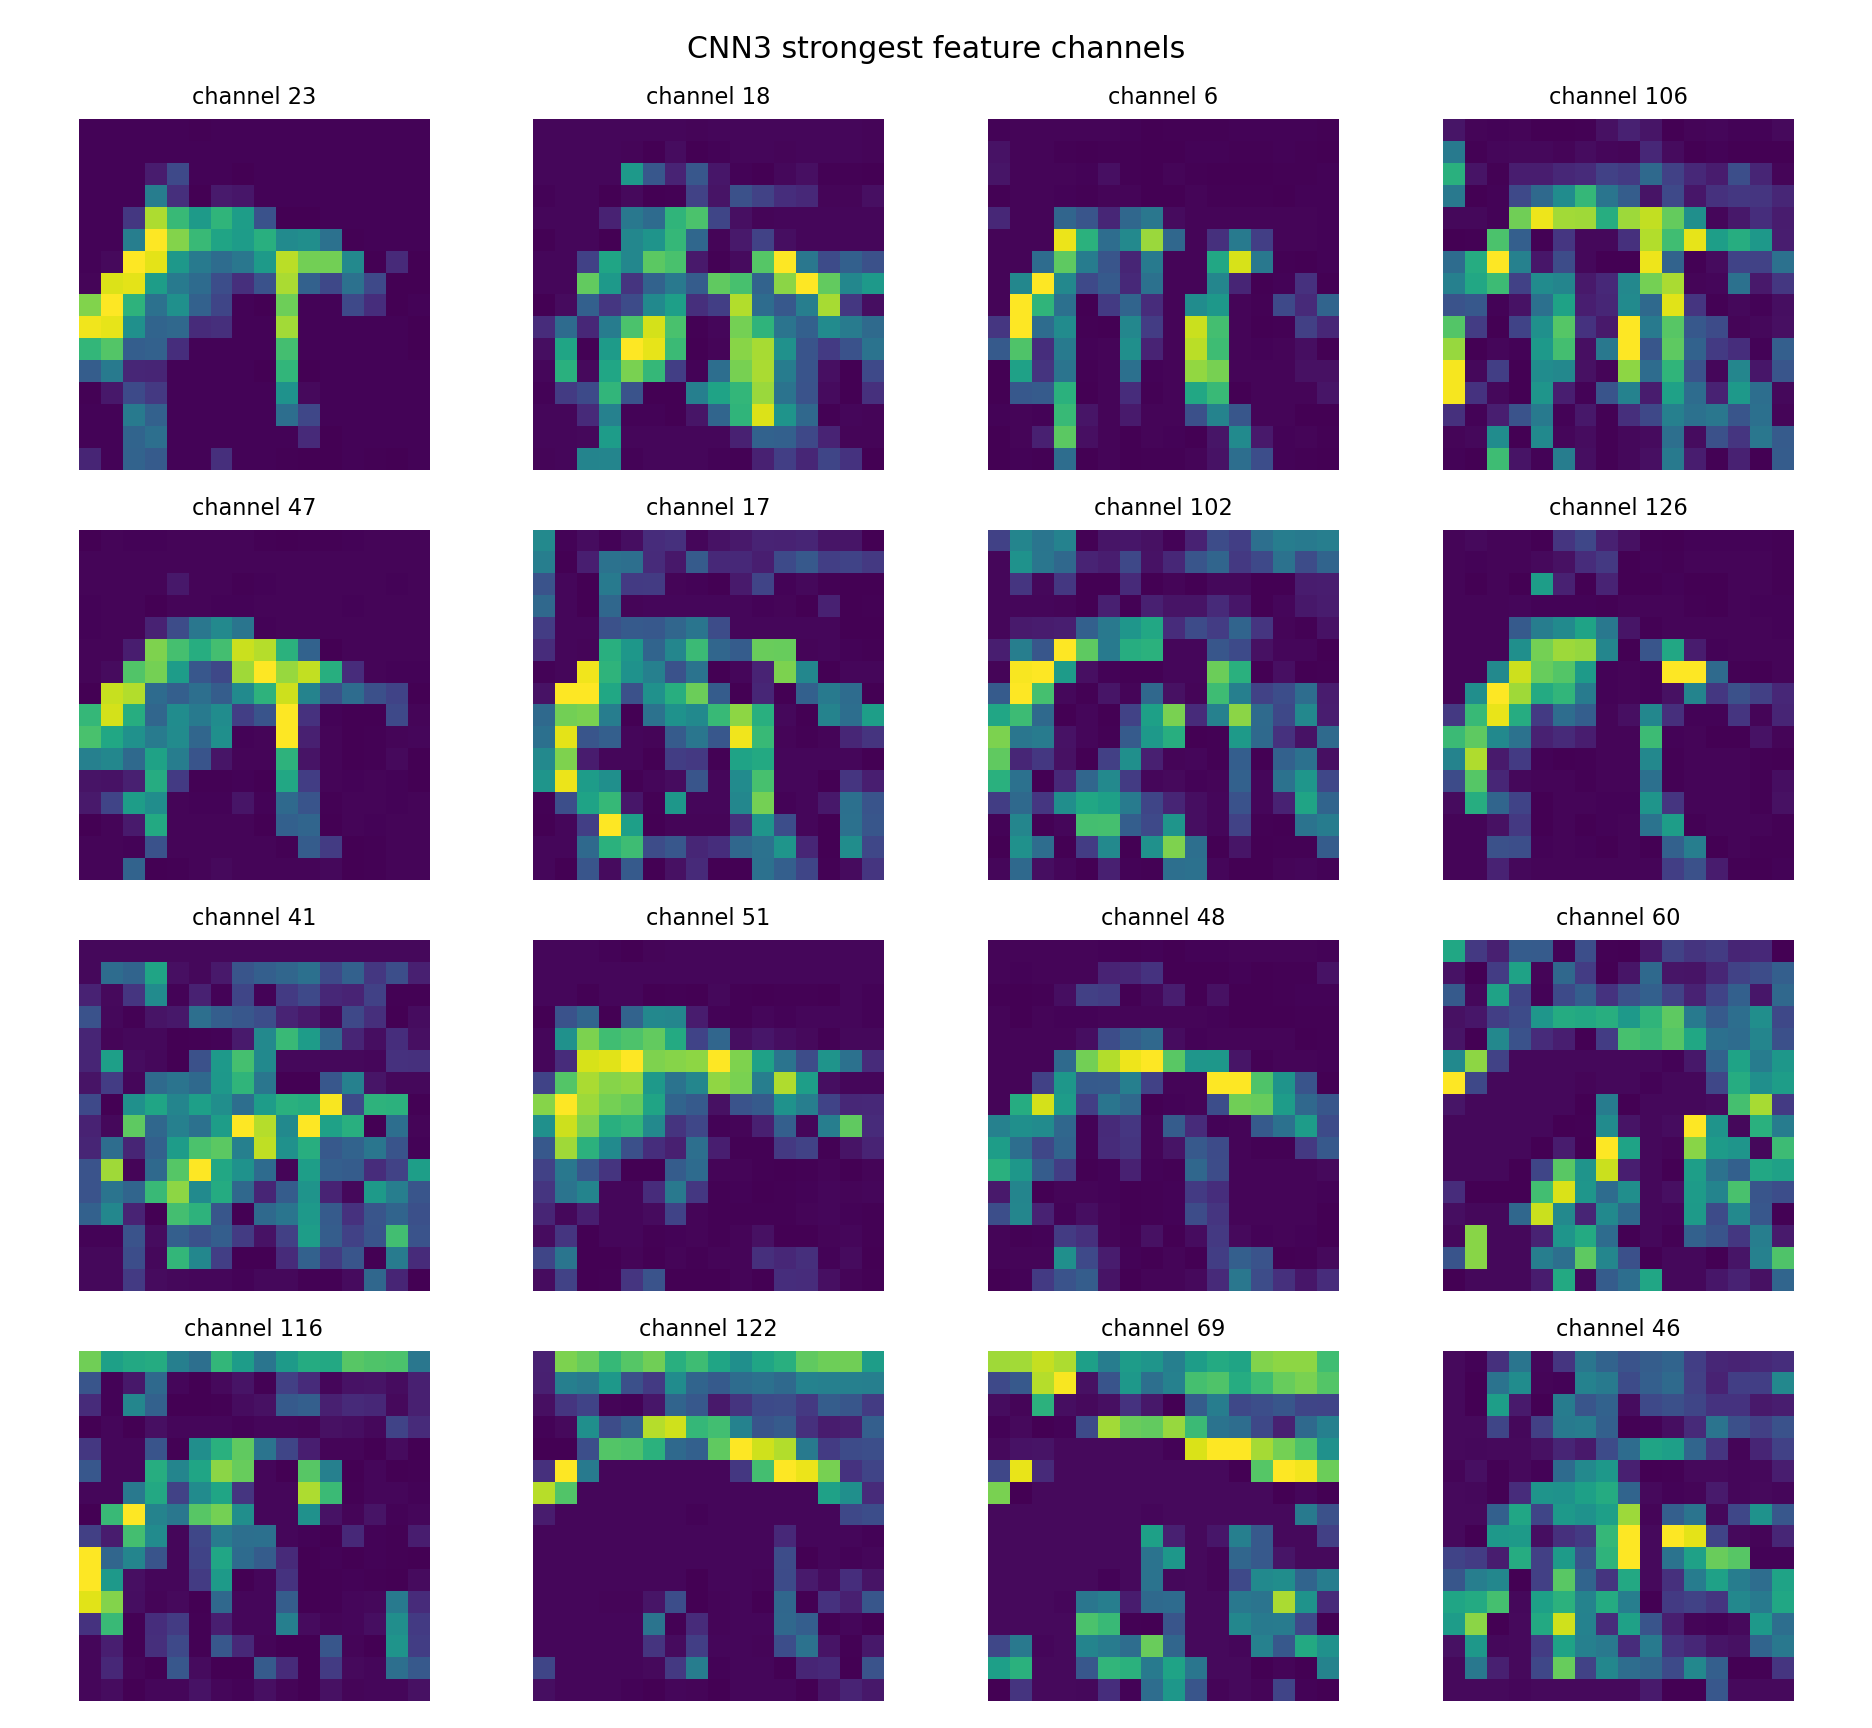
\includegraphics[width=\linewidth]{../visualizations/cnn3_voltages/validation_0/cnn3_top_channels.png}
  {\scriptsize\color{subtletext}
    Top CNN feature channels by mean absolute activation (validation sample 0).}
\end{column}
\end{columns}
\end{frame}

% ── SLIDE 11: Transformer Decoder Deep Dive ──────────────────────────────────
\begin{frame}[shrink=5]{Transformer Decoder: How the CLS Token Reads the Reservoir}
\begin{columns}[T]
\begin{column}{0.50\textwidth}
  \textbf{Pipeline for membrane\_transformer (702k):}
  \vspace{0.3em}
  {\scriptsize
  \begin{tabular}{ll}
    \toprule
    Step & Shape \\
    \midrule
    TPSAPU output (membrane) & $(B,256,512)$ \\
    LayerNorm + Linear(512$\to$128) & $(B,256,128)$ \\
    Prepend CLS token & $(B,257,128)$ \\
    + learned pos.\ embed & $(B,257,128)$ \\
    $\times2$ TransformerEncoderLayer & $(B,257,128)$ \\
    \quad 4 heads $\times$ 32 dims, 512-FFN & \\
    \quad Post-LN, GELU, bidirectional & \\
    Extract CLS + LayerNorm & $(B,128)$ \\
    Linear(128$\to$200) & $(B,200)$ \\
    \bottomrule
  \end{tabular}}
  \vspace{0.3em}
  \begin{itemize}\small
    \item CLS attends to \hl{all 256 TPSAPU-state positions}
    \item Each position $= $ one CNN spatial patch processed through the reservoir
    \item The transformer never sees pixels — it sees \textbf{spike/membrane histories}
    \item 4096$\to$128 for ResCNN: 32$\times$ compression before any attention
  \end{itemize}
\end{column}
\begin{column}{0.46\textwidth}
  \begin{tcolorbox}[mybox,title=What does CLS pay attention to?]
    \scriptsize
    \textbf{CNN3-702k:} L1 entropy $\approx$5.25 (max 5.55 for 256 tokens) —
    \hl{near-uniform} over all 256 positions. The decoder reads the whole image
    rather than fixating on specific patches.\\[0.4em]
    \textbf{Head specialization:} 4 heads focus on different image quadrants
    (bottom-right, top-right, left-center, right-center).
    Cosine similarity $\approx0.3$–0.6 between heads.\\[0.4em]
    \textbf{Layer refinement:} L2 is slightly \emph{more focused} on
    correct predictions (entropy $-0.04$ lower) — the second layer sharpens
    what L1 spread broadly.
  \end{tcolorbox}
  \vspace{0.3em}
  \begin{tcolorbox}[mybox,title=Comparison to ViT]
    \scriptsize
    ViT processes \emph{raw image patches} in its transformer.
    Here the transformer processes \hl{spiking neural activity patterns} —
    one step removed from pixels.
  \end{tcolorbox}
\end{column}
\end{columns}
\end{frame}

% ── SLIDE 12: CLS Attention Maps ─────────────────────────────────────────────
\begin{frame}[shrink=5]{CNN3-702k: Where the Transformer Looks (Aggregate, 500 Samples)}
\begin{columns}[T]
\begin{column}{0.50\textwidth}
  \centering
  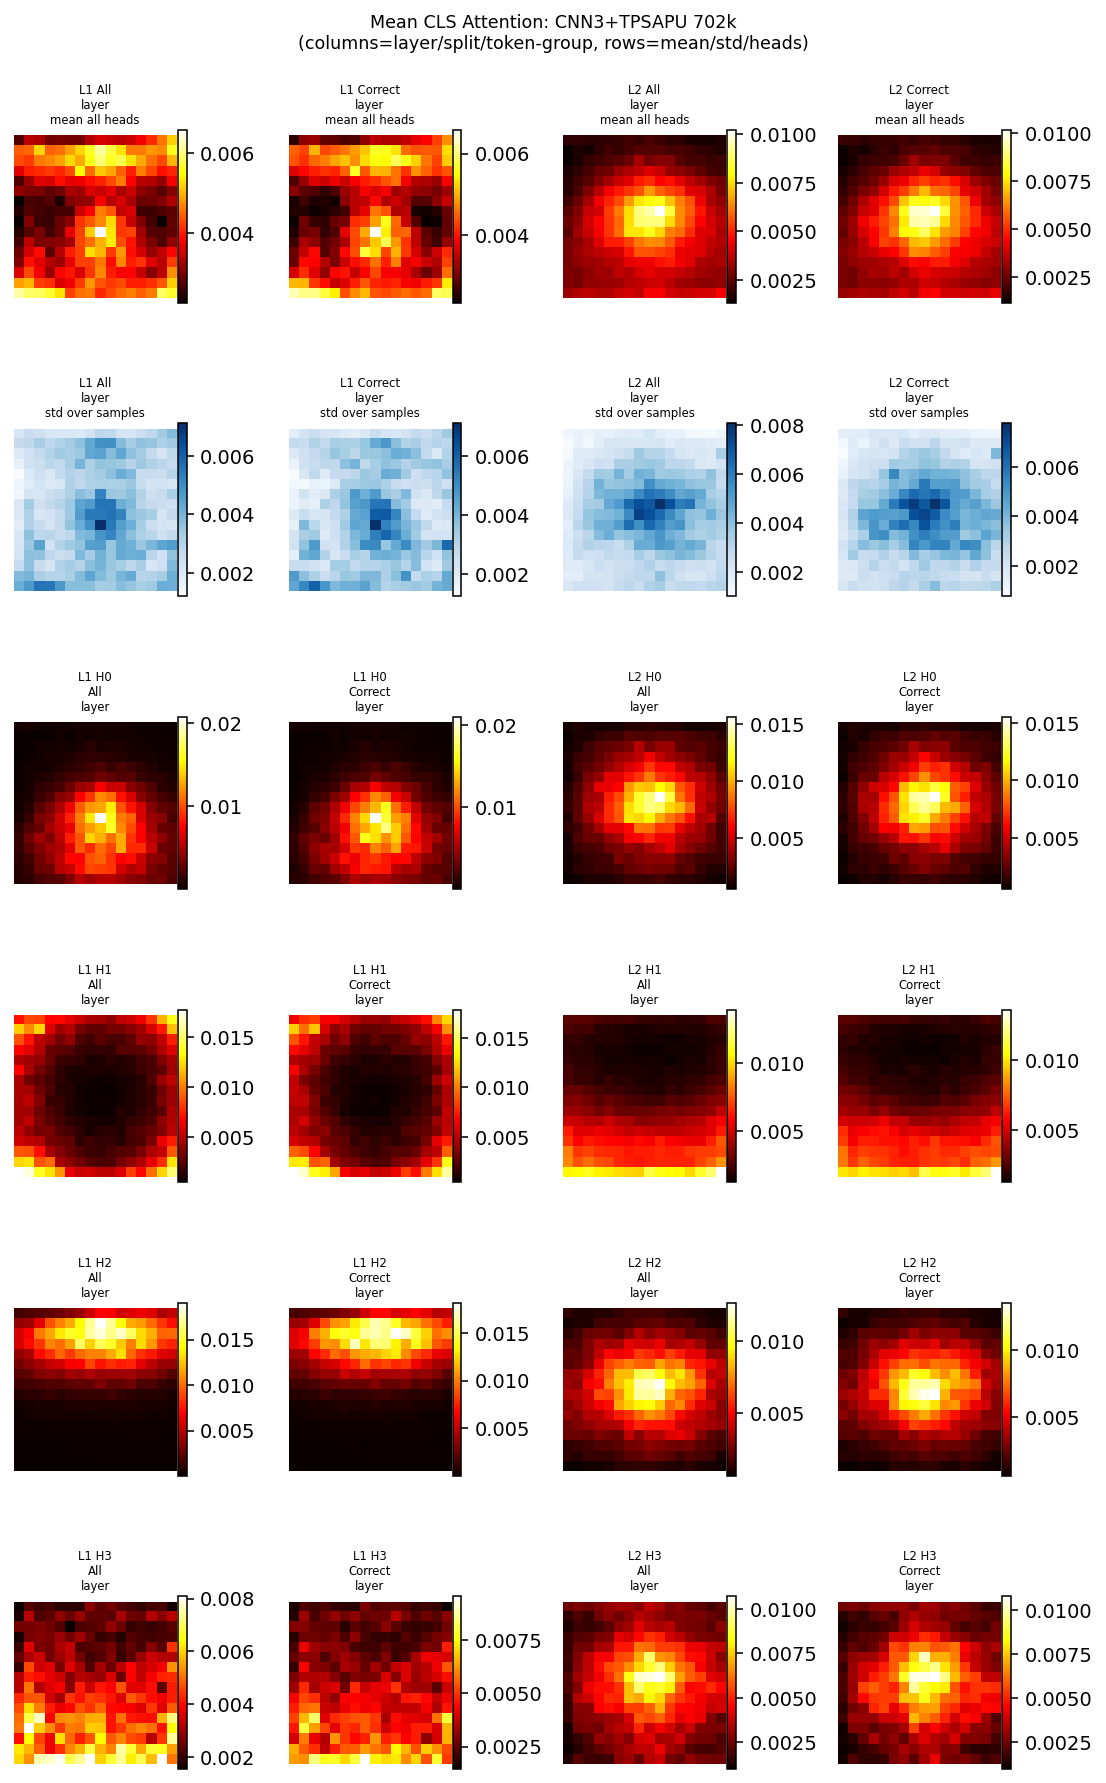
\includegraphics[width=\linewidth]{../visualizations/attention_analysis/cnn3_702k/mean_cls_attention.png}
  {\scriptsize\color{subtletext}
    Mean CLS attention over 500 val samples: all samples (top) and correct predictions only (bottom).\\
    Columns: mean over all heads, std, then per-head H0–H3.}
\end{column}
\begin{column}{0.46\textwidth}
  \centering
  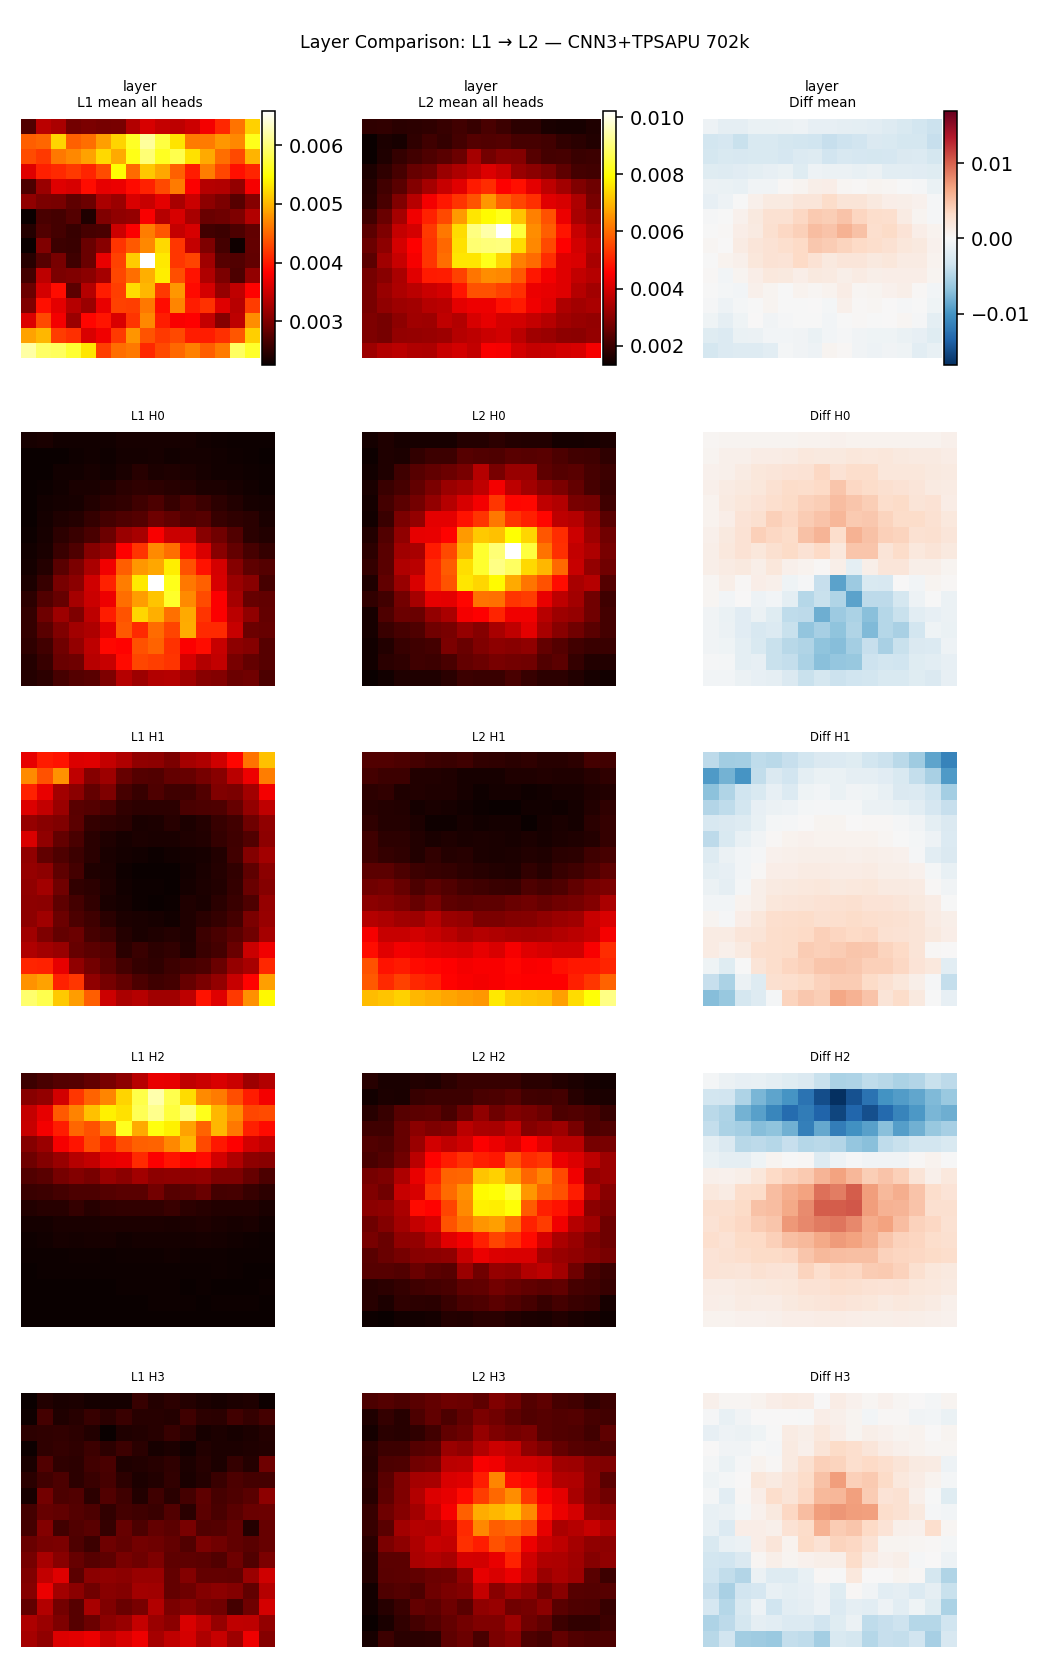
\includegraphics[width=\linewidth]{../visualizations/attention_analysis/cnn3_702k/layer_comparison.png}
  {\scriptsize\color{subtletext}
    Layer 1 (row 1), Layer 2 (row 2), difference L2$-$L1 (row 3).\\
    Red = L2 increases attention; Blue = L2 decreases.}
\end{column}
\end{columns}
\vspace{0.2em}
\begin{tcolorbox}[mybox]
  \scriptsize
  \textbf{Key finding:} attention is broadly spread (near-uniform), but
  Heads 0 and 3 develop mild preference for \hl{image corners and borders} —
  regions where the CNN produces the most distinctive token norms.
  L2 shifts weight slightly toward image centres relative to L1.
  \textbf{No single patch dominates} — the transformer aggregates the full reservoir context.
\end{tcolorbox}
\end{frame}

% ── SLIDE 13: Per-Image Attention Overlay ────────────────────────────────────
\begin{frame}{CNN3-702k: Attention Overlaid on Individual Validation Images}
\centering
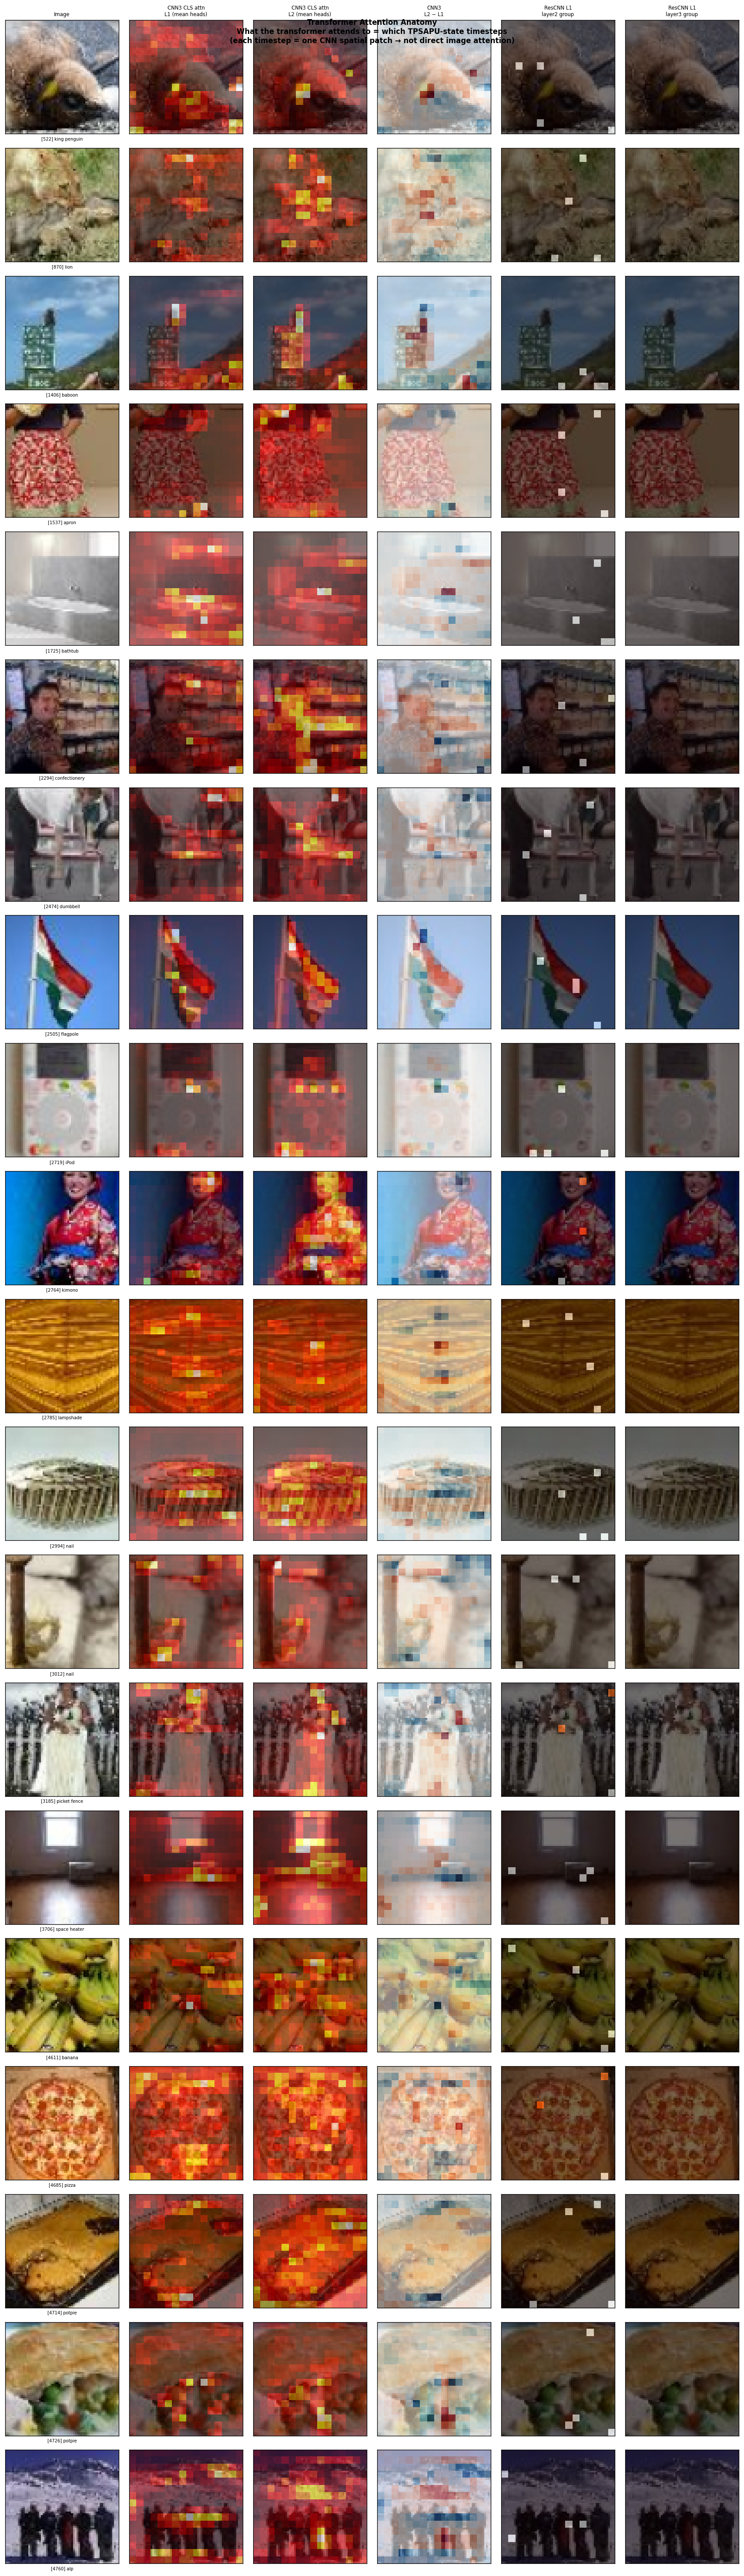
\includegraphics[height=0.78\textheight,width=\linewidth,keepaspectratio]{../visualizations/validation_20/attention_anatomy.png}
\vspace{0.15em}
{\tiny\color{subtletext}
  Cols: image $\mid$ CNN3 L1 $\mid$ CNN3 L2 $\mid$ L2$-$L1 diff $\mid$ ResCNN layer2 $\mid$ ResCNN layer3 (un-normalized — note sparse attention).
  Heat = CLS attention to TPSAPU states at that CNN spatial patch.}
\end{frame}

% ── SLIDE 14: The Fun Fail ────────────────────────────────────────────────────
\begin{frame}{\red{The Fun Fail}: ResCNN Layer3 Was Never Normalized}
\begin{columns}[T]
\begin{column}{0.50\textwidth}
  \centering
  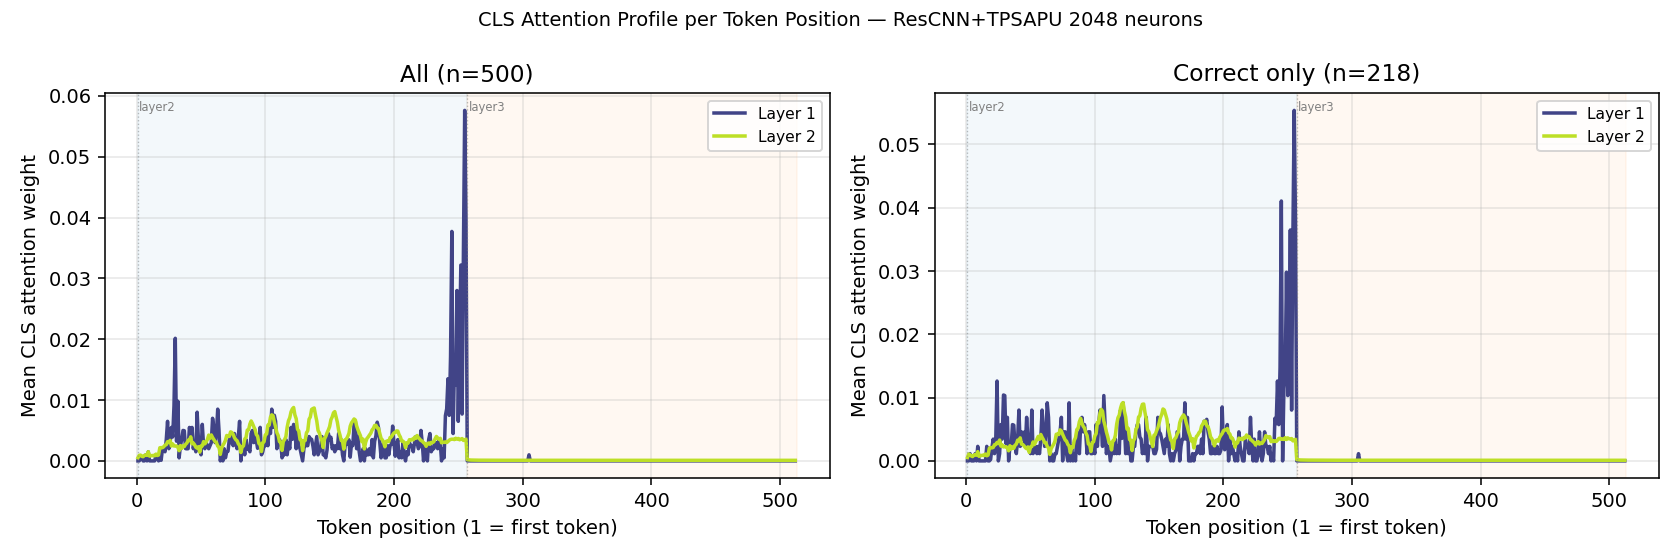
\includegraphics[width=\linewidth]{../visualizations/attention_analysis/rescnn_2048/positional_attention_profile.png}
  {\scriptsize\color{subtletext}
    CLS attention profile across all 512 token positions.
    Tokens 0–255 = res\_cnn layer2. Tokens 256–511 = \red{layer3 (un-normalized)}.}
\end{column}
\begin{column}{0.46\textwidth}
  \begin{tcolorbox}[failbox,title=What happened]
    \scriptsize
    \textbf{res\_cnn layer3} is a residual refinement:
    \texttt{layer3 = layer2 + conv3(layer2)}\\[0.2em]
    \textbf{No LayerNorm added.} Layer3 magnitudes are \red{much larger}.
    When fed into TPSAPU, many neurons immediately exceed threshold and
    \red{spike like crazy} — high-frequency noise rather than signal.
  \end{tcolorbox}
  \vspace{0.15em}
  \begin{exampleblock}{But the model still works!}
    \scriptsize
    The transformer \hl{learned to ignore} tokens 256–511:
    L1 attention is \textbf{essentially zero} for all layer3 positions.
    L2 corrects by spreading attention more uniformly.\\[0.1em]
    Top-1: \textbf{39.2\%} despite half the tokens being useless.\\
    \textit{Imagine the potential with normalized layer3 + more training!}
  \end{exampleblock}
\end{column}
\end{columns}
\end{frame}

% ── SLIDE 15: Scaling to ImageNet ────────────────────────────────────────────
\begin{frame}[shrink=8]{Scaling Up: Three Models on Tiny ImageNet (200 classes, 64$\times$64)}
\begin{columns}[T]
\begin{column}{0.46\textwidth}
  {\scriptsize
  \renewcommand{\arraystretch}{1.25}
  \begin{tabular}{lcc}
    \toprule
    & \textbf{MNIST} & \textbf{Tiny ImageNet} \\
    \midrule
    Classes & 10 & \hl{200} \\
    Resolution & 28$^2$ & \hl{64$^2$, 3ch} \\
    CNN tokens & 49 & \hl{256 or 512} \\
    Taus & 3 & \hl{8} \\
    $d_\text{res}$ & 64 & 64 or 256 \\
    Neurons & 192 & \hl{512 or 2048} \\
    Training & 20 ep & \hl{40–104 ep} \\
    \bottomrule
  \end{tabular}}
  \vspace{0.5em}
  \begin{tcolorbox}[mybox,title={\orange{ResNet-18} baseline}]
    \scriptsize 11.28M params, tiny stem ($3\times3$, no maxpool),
    AdamW, 40 epochs. Strong spatial inductive bias.
  \end{tcolorbox}
  \vspace{0.25em}
  \begin{tcolorbox}[mybox,title={\blue{CNN3+TPSAPU 702k}}]
    \scriptsize CNN3 encoder, TPSAPU (512 neurons, 8$\tau$),
    Membrane-Transformer. 95\% pruning target, 104 epochs.
  \end{tcolorbox}
  \vspace{0.25em}
  \begin{tcolorbox}[mybox,title={\green{ResCNN+TPSAPU 2048}}]
    \scriptsize ResCNN encoder, CrossReservoir TPSAPU (2048 neurons),
    Both-Transformer. 63/85 epochs — \red{training interrupted}.
  \end{tcolorbox}
\end{column}
\begin{column}{0.50\textwidth}
  \centering
  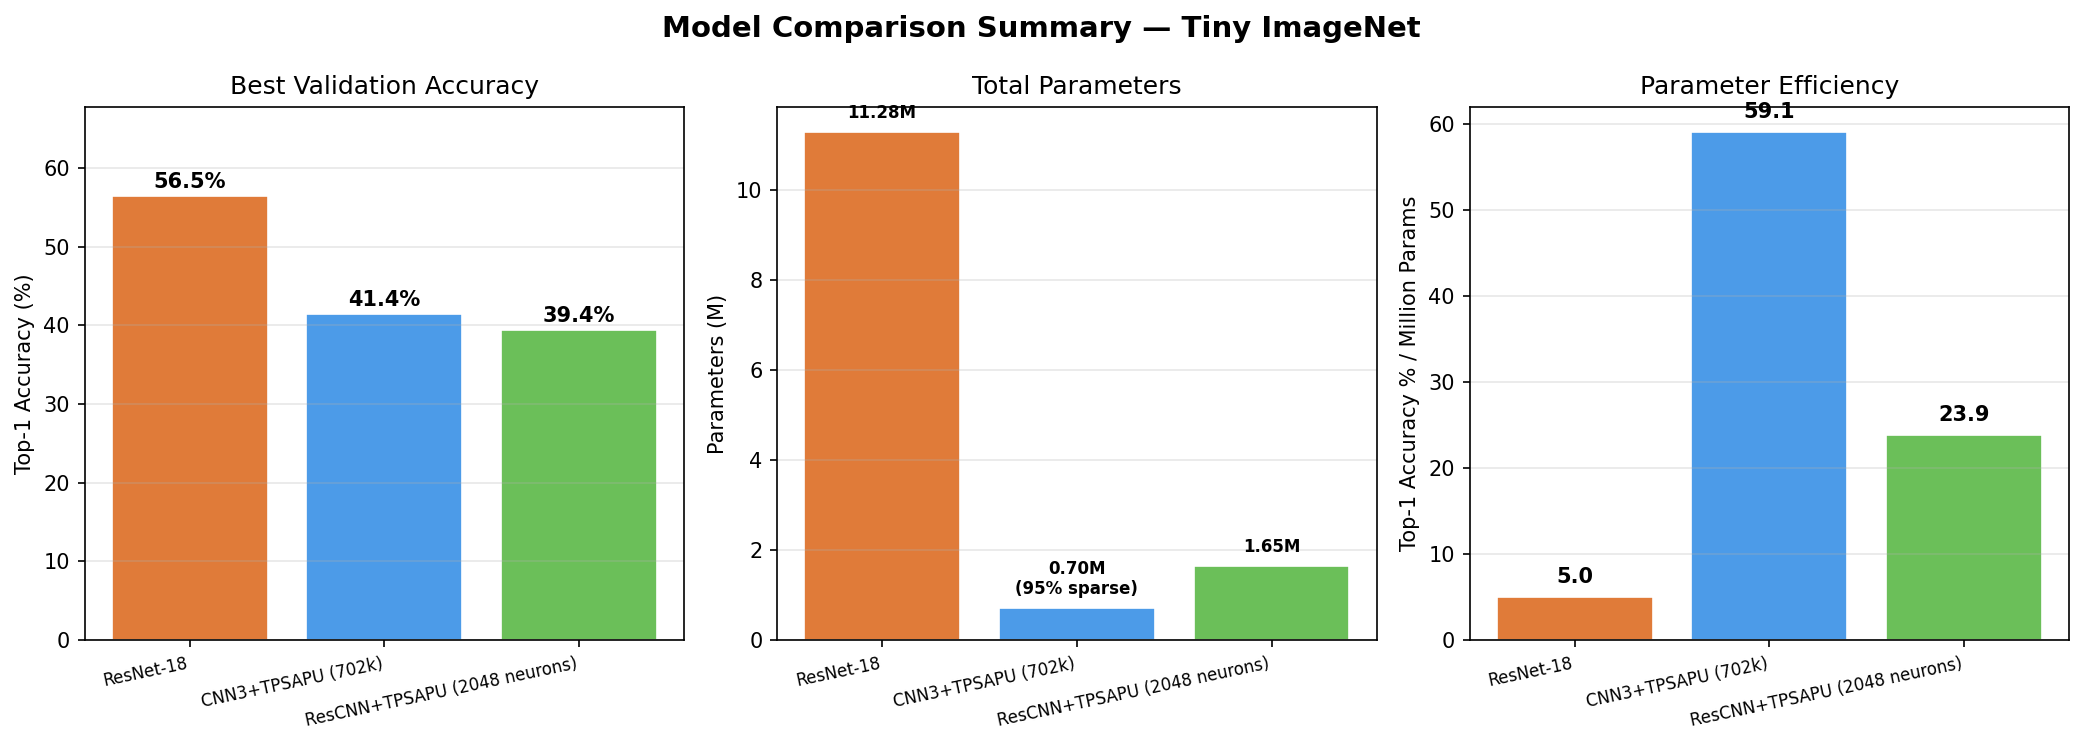
\includegraphics[width=\linewidth]{../visualizations/comparison/02_model_summary.png}
\end{column}
\end{columns}
\end{frame}

% ── SLIDE 16: Training Dynamics ──────────────────────────────────────────────
\begin{frame}[shrink=14]{Training Dynamics: All Three Models}
\centering
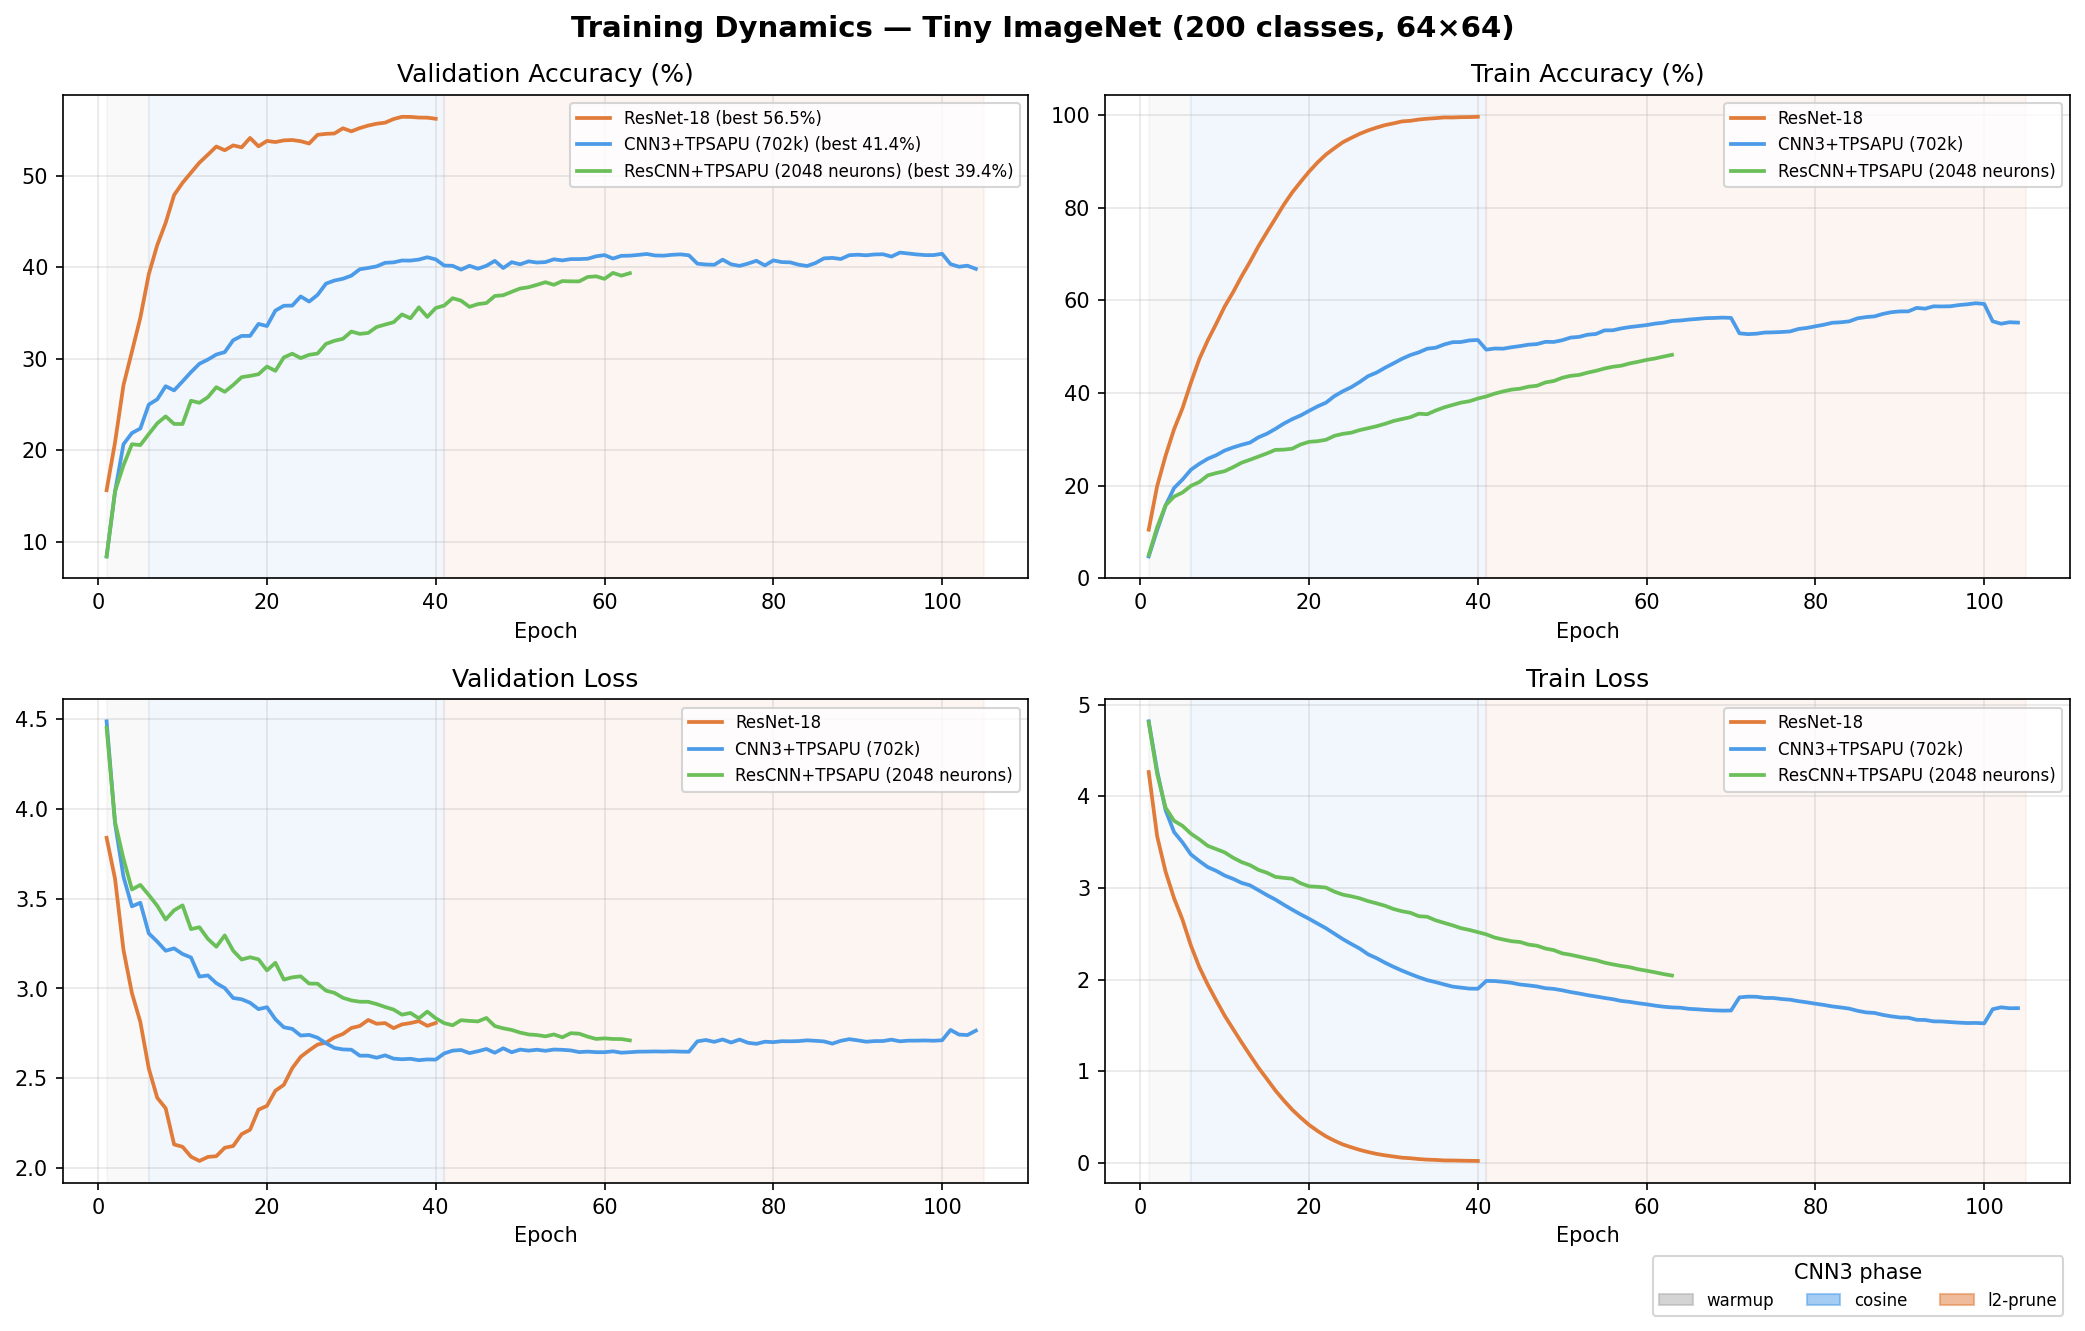
\includegraphics[
  width=0.68\linewidth,
  height=0.55\textheight,
  keepaspectratio
]{../visualizations/comparison/01_training_curves.png}
\vspace{0.15em}
\begin{columns}[T]
\begin{column}{0.32\textwidth}
  \begin{tcolorbox}[mybox,colframe=accent0!60]
    \fontsize{5.5}{6.2}\selectfont \orange{ResNet-18}: fast convergence, strong overfit (train 99\% vs val 57\%)
  \end{tcolorbox}
\end{column}
\begin{column}{0.32\textwidth}
  \begin{tcolorbox}[mybox,colframe=accent1!60]
    \fontsize{5.5}{6.2}\selectfont \blue{CNN3-702k}: l2-prune phase visible as mild dip then recovery; far less overfit
  \end{tcolorbox}
\end{column}
\begin{column}{0.32\textwidth}
  \begin{tcolorbox}[mybox,colframe=accent2!60]
    \fontsize{5.5}{6.2}\selectfont \green{ResCNN-2048}: 63/85 epochs; small batch (8) slows convergence
  \end{tcolorbox}
\end{column}
\end{columns}
\end{frame}

% ── SLIDE 17: Efficiency ─────────────────────────────────────────────────────
\begin{frame}[shrink=10]{Efficiency: 12$\times$ More Accuracy per Parameter}
\begin{columns}[T]
\begin{column}{0.50\textwidth}
  \centering
  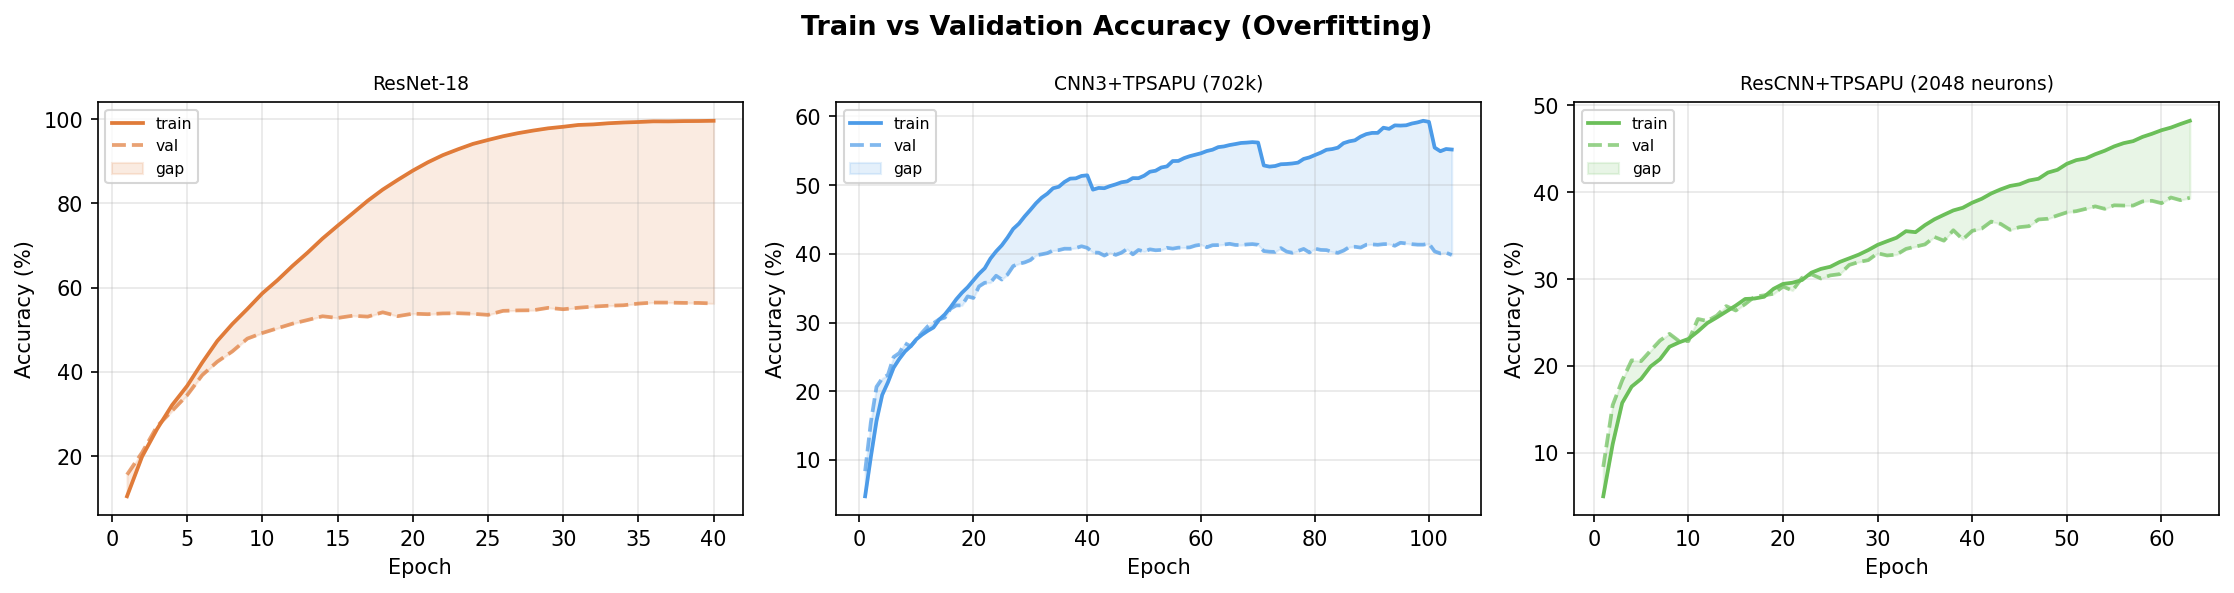
\includegraphics[width=\linewidth]{../visualizations/comparison/09_overfit_analysis.png}
  {\scriptsize\color{subtletext}
    Train (solid) vs val (dashed). TPSAPU models overfit far less.}
\end{column}
\begin{column}{0.46\textwidth}
  {\scriptsize\renewcommand{\arraystretch}{1.3}
  \begin{tabular}{lccc}
    \toprule
    Model & Params & Top-1 & Acc/M \\
    \midrule
    \orange{ResNet-18} & 11.28M & \textbf{56.7\%} & 5.0 \\
    \blue{CNN3-702k}   & 0.70M  & 41.6\% & \hl{59.3} \\
    \green{RCN-2048}   & 1.65M  & 39.2\% & 23.8 \\
    \bottomrule
  \end{tabular}}
  \vspace{0.4em}
  \begin{block}{Parameter efficiency}
    CNN3-702k achieves \hl{59.3 acc\%/M params}\\
    vs 5.0 for ResNet-18 — \textbf{12$\times$ more efficient}
  \end{block}
  \vspace{0.3em}
  \begin{tcolorbox}[mybox]
    \scriptsize
    TPSAPU's implicit regularization (dropout, sparse recurrent,
    binary spikes) prevents the extreme overfit seen in ResNet-18
    (train 99\% → val 57\%).
    The TPSAPU gap (train$-$val) stays $<$15pp.
  \end{tcolorbox}
\end{column}
\end{columns}
\end{frame}

% ── SLIDE 18: Pruning ────────────────────────────────────────────────────────
\begin{frame}{95\% Sparsity with Only Minor Accuracy Loss}
\centering
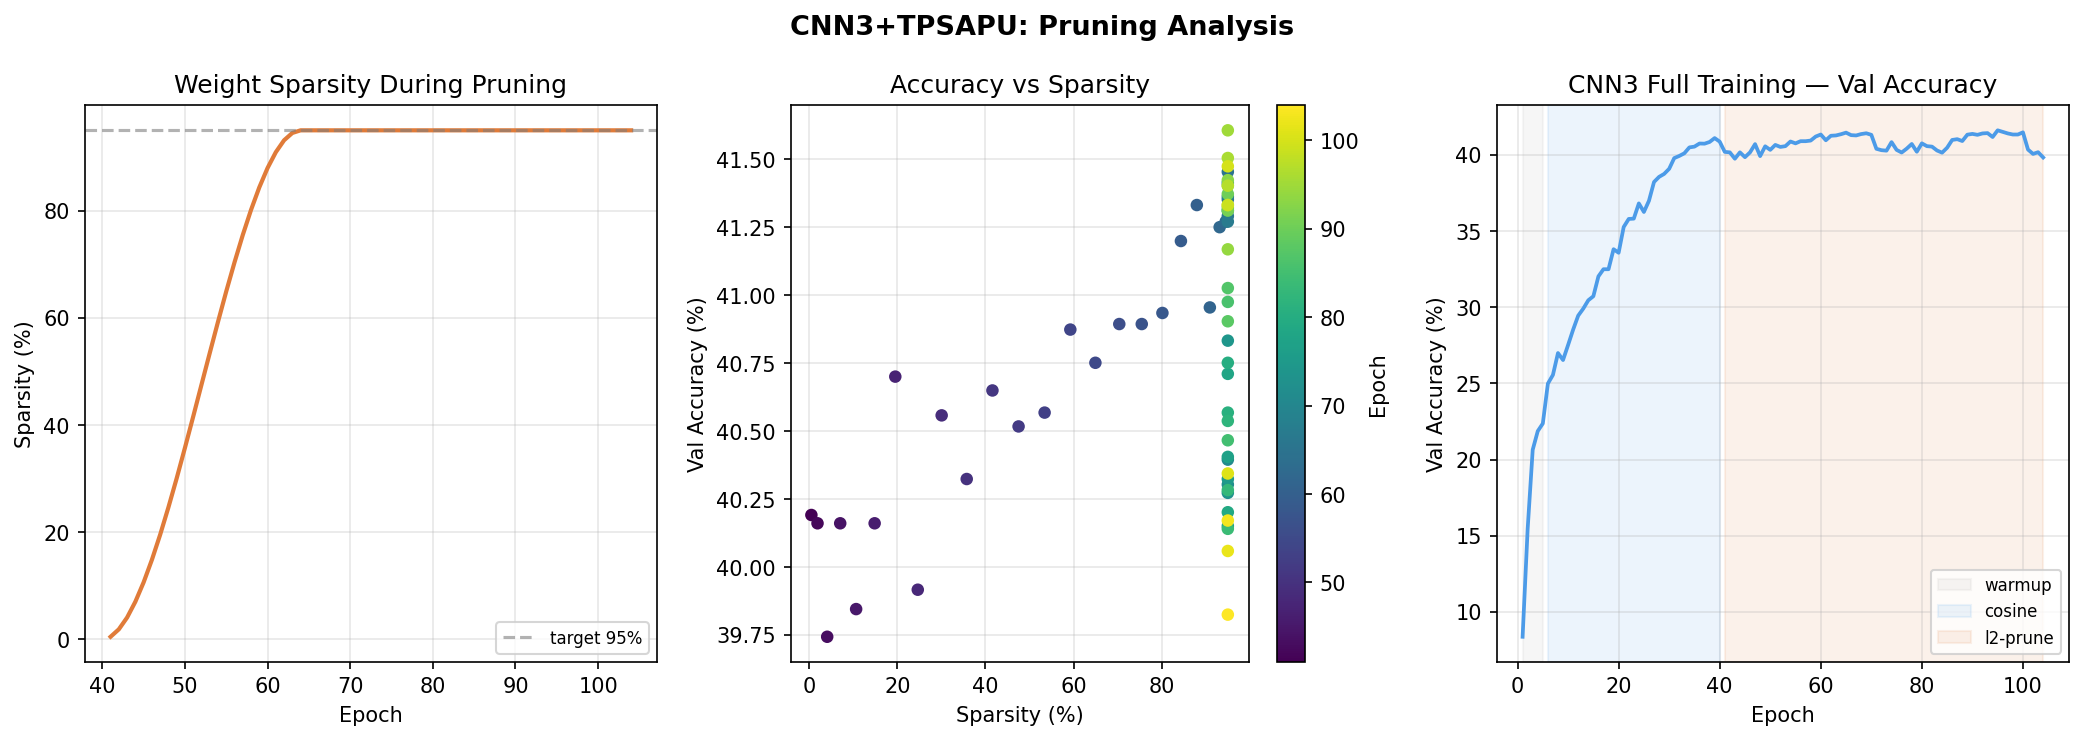
\includegraphics[width=0.92\linewidth]{../visualizations/comparison/03_sparsity_analysis.png}
\vspace{0.3em}
\begin{columns}[T]
\begin{column}{0.32\textwidth}
  \begin{tcolorbox}[mybox]
    \scriptsize
    L2 pressure ramps over 24 epochs, then 6 epochs stabilize at the 95\% mask.
  \end{tcolorbox}
\end{column}
\begin{column}{0.32\textwidth}
  \begin{block}{Accuracy drop}
    \scriptsize Dips during aggressive pruning then partially recovers in stabilization.
  \end{block}
\end{column}
\begin{column}{0.32\textwidth}
  \begin{exampleblock}{Key result}
    \scriptsize \hl{41.6\% top-1 with only 5\% of recurrent weights non-zero.} Ideal for hardware.
  \end{exampleblock}
\end{column}
\end{columns}
\end{frame}

% ── SLIDE 19: Per-Class ──────────────────────────────────────────────────────
\begin{frame}{Per-Class Analysis: 200 Classes, 4909 Validation Samples}
\begin{columns}[T]
\begin{column}{0.50\textwidth}
  \centering
  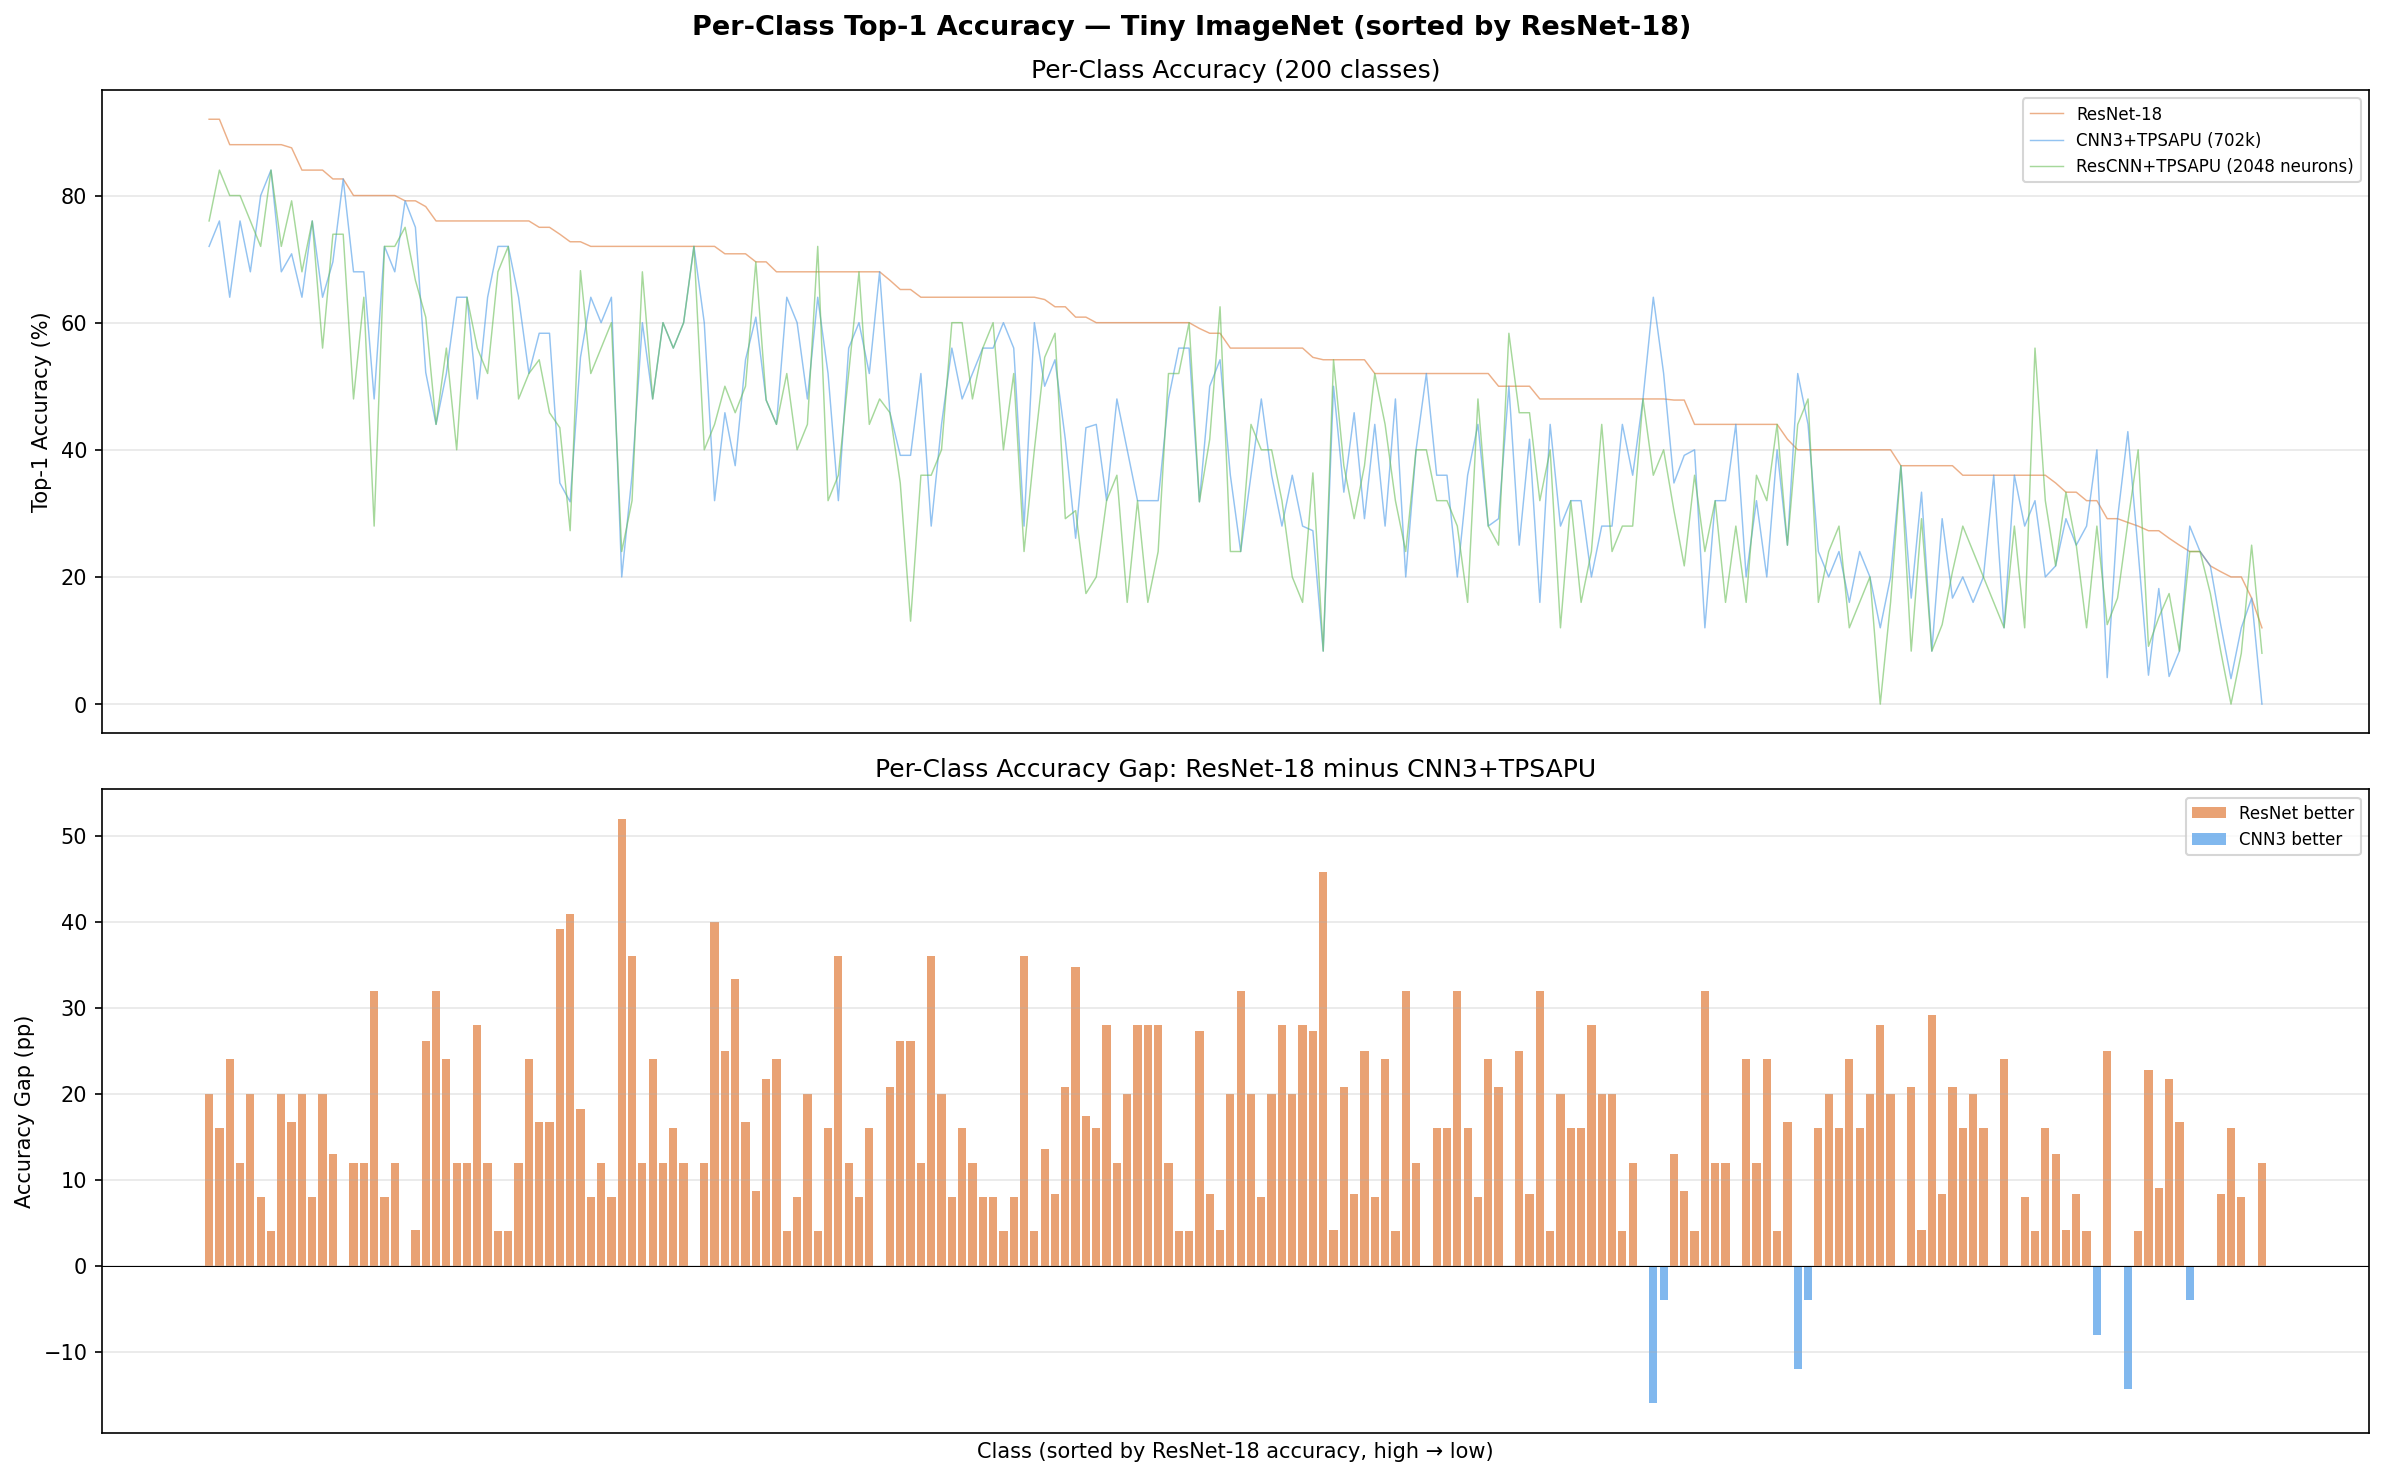
\includegraphics[width=\linewidth]{../visualizations/comparison/04_per_class_accuracy.png}
  {\scriptsize\color{subtletext}
    Classes sorted by ResNet-18 accuracy. Lower panel: accuracy gap ResNet minus CNN3.}
\end{column}
\begin{column}{0.46\textwidth}
  \begin{itemize}\small
    \item All models fail on the \emph{same} hard classes (fine-grained species, similar textures)
    \item Easy classes (goldfish, pizza, alp): all models $>$85\%
    \item CNN3-702k \hl{beats ResNet-18 on specific classes} despite 16$\times$ fewer params
    \item Top-5: ResNet 79.2\% | CNN3 67.6\% | ResCNN 65.4\%
    \item TPSAPU top-5/top-1 ratio: $1.63\times$ vs $1.40\times$ for ResNet\\
          (more uncertain but top-5 competitive)
  \end{itemize}
  \vspace{0.3em}
  \begin{tcolorbox}[mybox]
    \scriptsize
    The per-class confusion structure is \textbf{similar across models} — difficulty is
    mostly in the data (64px thumbnails of 200 classes), not the architecture.
  \end{tcolorbox}
\end{column}
\end{columns}
\end{frame}

% ── SLIDE 20: ResNet Effective Rank ──────────────────────────────────────────
\begin{frame}{ResNet-18 Internal Analysis: Effective Rank per Layer}
\begin{columns}[T]
\begin{column}{0.50\textwidth}
  \centering
  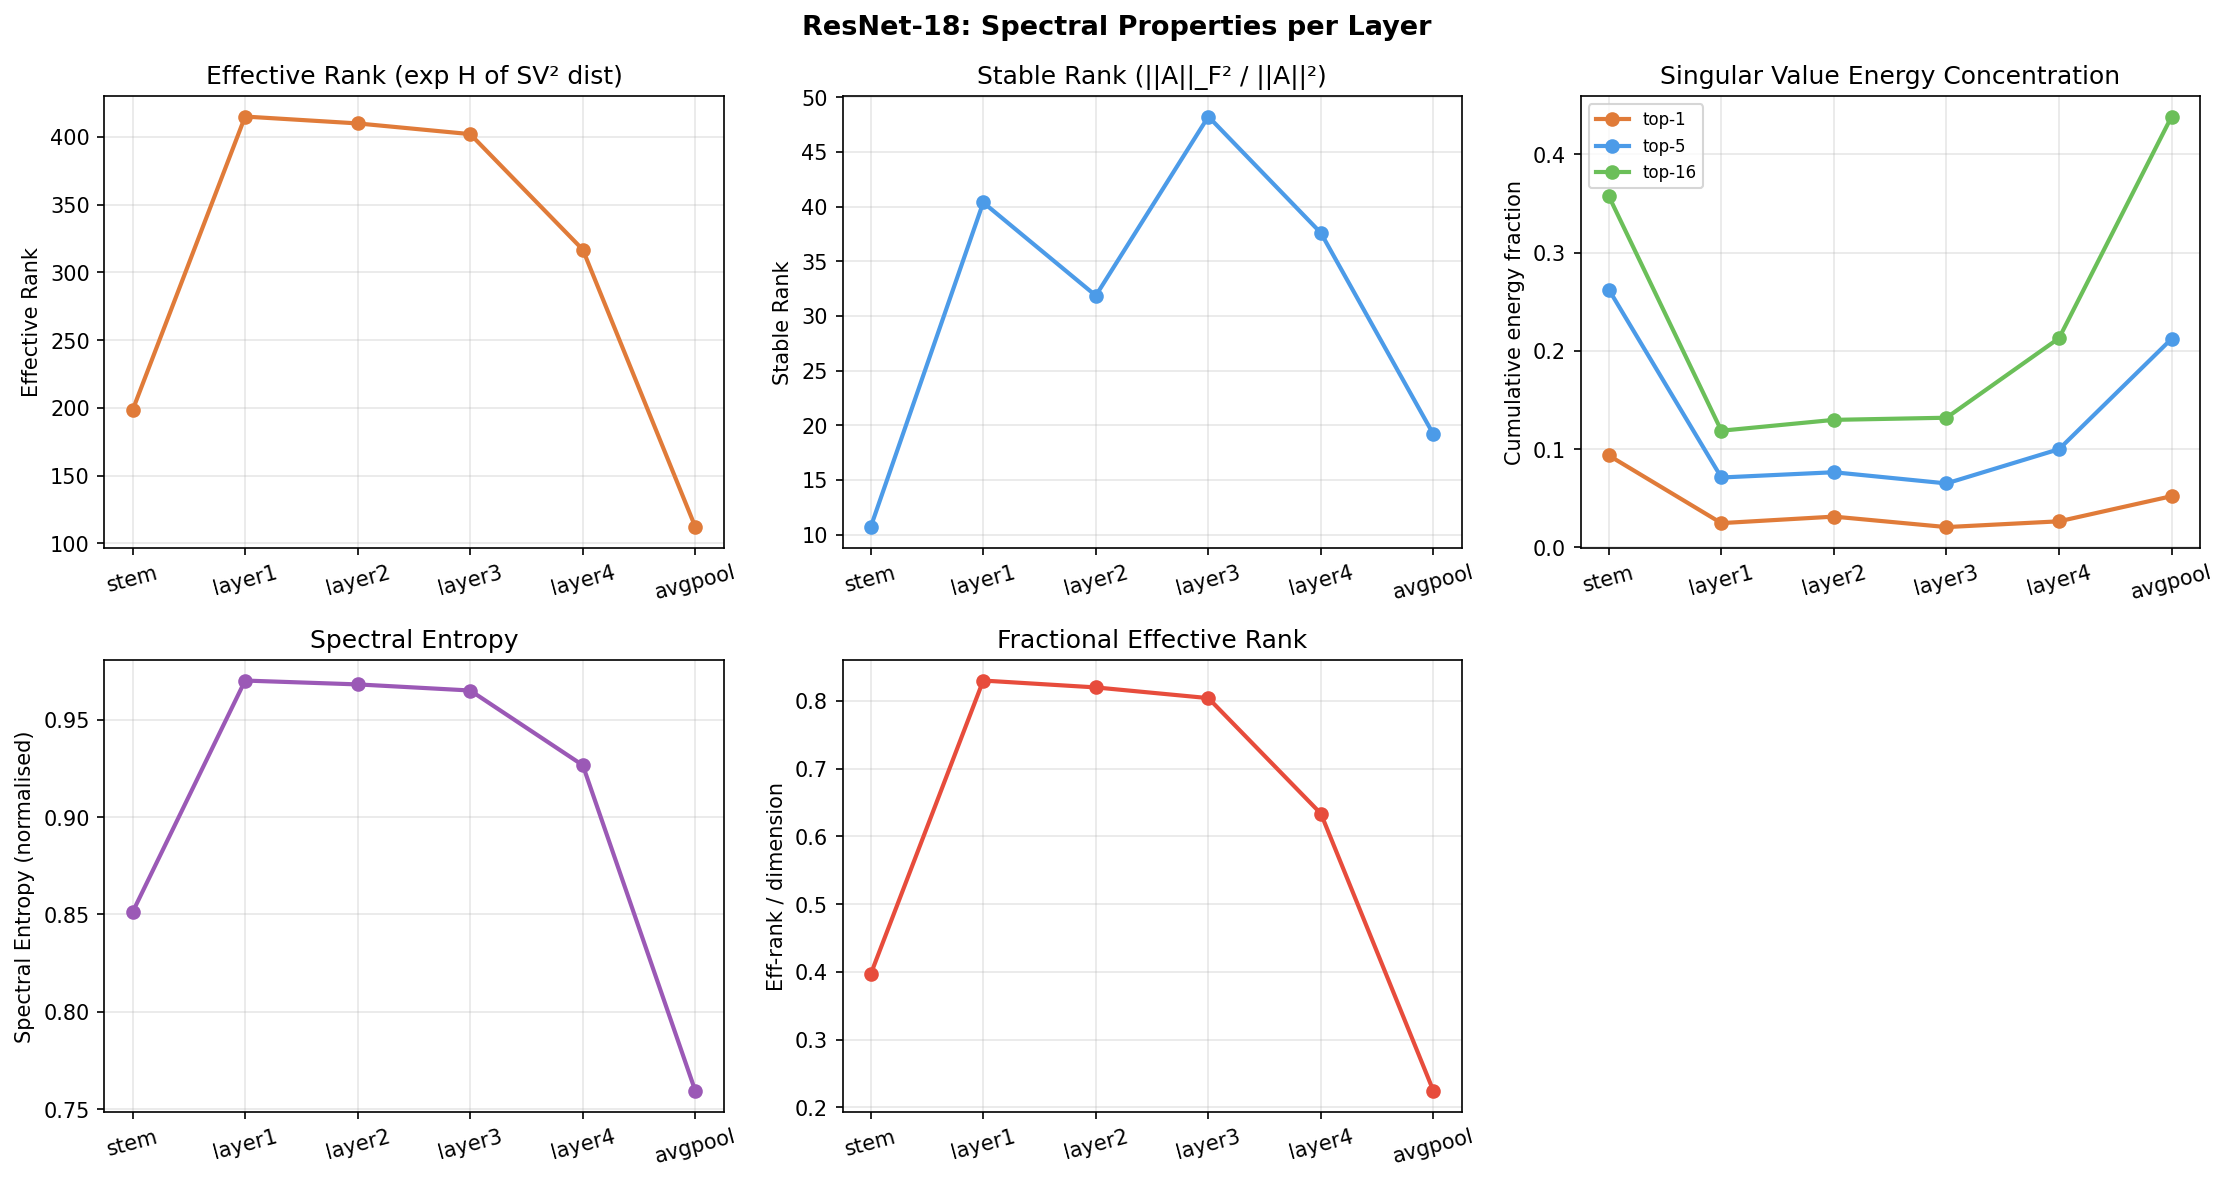
\includegraphics[width=\linewidth]{../visualizations/resnet18/effective_rank_per_layer.png}
\end{column}
\begin{column}{0.46\textwidth}
  \textbf{Eff.\ rank} $= e^H$, $H = -\textstyle\sum_i p_i \ln p_i$, $p_i = \sigma_i^2/\|\sigma\|^2$
  \vspace{0.4em}
  {\scriptsize\renewcommand{\arraystretch}{1.2}
  \begin{tabular}{lrr}
    \toprule
    Layer & Eff.\ Rank & Top-1 E \\
    \midrule
    stem    & 198 & 9.4\% \\
    layer1  & \hl{415} & 2.5\% \\
    layer2  & 410 & 3.1\% \\
    layer3  & 402 & 2.1\% \\
    layer4  & 317 & 2.7\% \\
    avgpool & \orange{112} & 5.2\% \\
    \bottomrule
  \end{tabular}}
  \vspace{0.3em}
  \begin{tcolorbox}[mybox]
    \scriptsize
    Middle layers span \emph{almost the full sample space} (eff.\ rank 400/500).
    avgpool \hl{bottlenecks} to 112 — strong overfit: the huge intermediate capacity maps
    to a narrow final representation.\\[0.3em]
    TPSAPU is structurally different: the reservoir is a \hl{fixed-dim bottleneck}
    that never expands — no intermediate overfit pathway.
  \end{tcolorbox}
\end{column}
\end{columns}
\end{frame}


% ── SLIDE 21: TPSAPU Effective Rank / Redundancy ────────────────────────────
\begin{frame}[shrink=8]{TPSAPU Effective Rank: Redundant, Low-Dimensional, Still Working}
\centering


\includegraphics[
  width=0.96\linewidth,
  height=0.24\textheight,
  keepaspectratio
]{/home/mateusz/sapu-psi-logs/visualizations/tpsapu_effective_rank/activation_effective_rank.png}

\vspace{0.1em}


\includegraphics[
  width=0.96\linewidth,
  height=0.30\textheight,
  keepaspectratio
]{/home/mateusz/sapu-psi-logs/visualizations/tpsapu_effective_rank/comparison_with_resnet.png}

\vspace{0.15em}

\begin{tcolorbox}[mybox,title=Why it still matters,width=0.96\linewidth]
\tiny
\begin{minipage}[t]{0.32\linewidth}
\textbf{Redundant reservoir.}
The TPSAPU activations have much lower fractional effective rank than ResNet-18 layers.
Even with a larger reservoir, the effective rank stays around 9--12.
\end{minipage}
\hfill
\begin{minipage}[t]{0.32\linewidth}
\textbf{Bloated matrix.}
This suggests that many neurons encode correlated directions.
The recurrent matrix may be oversized: wider reservoirs do not automatically create independent features.
\end{minipage}
\hfill
\begin{minipage}[t]{0.32\linewidth}
\textbf{Still functional.}
This is not a complete failure mode. The decoder can still extract class signal from the compact subspace,
so the reservoir acts like a strong regularizing bottleneck.
\end{minipage}
\end{tcolorbox}
\end{frame}

% ── SLIDE 22: FPGA & Neuromorphic Hardware ───────────────────────────────────
\begin{frame}[shrink=12]{Future: FPGA \& Neuromorphic Hardware}
\begin{columns}[T]
\begin{column}{0.48\textwidth}
  \begin{block}{Why \tpsapu{} maps naturally to hardware}
    \begin{itemize}\small
      \item \hl{Binary spikes} — multiply becomes wire-and-gate
      \item \hl{95\% sparse $W_\text{rec}$} — CSR format, 95\% fewer ops
      \item \hl{Streaming tokens} — one step at a time, unroll pipeline
      \item Shared $W_\text{rec}$ across all $\tau$s — one BRAM block
      \item Low-rank cross-reservoir ($r{=}16$) — tiny extra cost
      \item Fixed-point LIF membrane: 16-bit sufficient
    \end{itemize}
  \end{block}
  \vspace{0.3em}
  \begin{alertblock}{Neuromorphic targets}
    \begin{itemize}\scriptsize
      \item \textbf{Intel Loihi 2} — LIF neurons, on-chip learning
      \item \textbf{BrainScaleS-2} — analog membrane dynamics
      \item \textbf{SpiNNaker 2} — massively parallel spike routing
    \end{itemize}
  \end{alertblock}
\end{column}
\begin{column}{0.48\textwidth}
  \begin{exampleblock}{Estimated hardware gains}
    \begin{itemize}\scriptsize
      \item Dense CNN: all layers active every cycle
      \item \tpsapu{} at 95\% sparse + 10\% spike rate:
            $\approx\mathbf{0.5\%}$ of multiply-adds remain
      \item Token-streaming: latency $\propto$ sequence length,
            not image width — natural for edge sensors
      \item FPGA prototype target: $<$1W for 512-neuron model
    \end{itemize}
  \end{exampleblock}
  \vspace{0.2em}
  \begin{tcolorbox}[mybox,title=Short-term roadmap]
    \scriptsize
    1.~Quantization-aware training (INT8/INT16)\quad
    2.~Export pruned $W_\text{rec}$ as CSR\\
    3.~Implement LIF step in VHDL/HLS\quad
    4.~Benchmark vs Arm Ethos / Synaptics Orca
  \end{tcolorbox}
\end{column}
\end{columns}
\end{frame}

% ── SLIDE 23: Event-Based Processing ─────────────────────────────────────────
\begin{frame}[shrink=10]{Future: Event-Based Processing \& Dynamic Vision Sensors}
\begin{columns}[T]
\begin{column}{0.50\textwidth}
  \begin{block}{Why \tpsapu{} is a natural fit for event cameras}
    \begin{itemize}\small
      \item \textbf{DVS cameras} emit events $(x,y,t,\text{polarity})$ asynchronously
      \item Dense CNNs process fixed-size frames — \hl{mismatched representation}
      \item \tpsapu{} already processes a \hl{token sequence} of variable length
      \item Events can be tokenized spatially ($\to$ CNN patches) or temporally ($\to$ time bins)
      \item \hl{Sparse events} $\leftrightarrow$ \hl{sparse spikes}: both architecturally aligned
    \end{itemize}
  \end{block}
  \vspace{0.3em}
  \begin{tcolorbox}[mybox,title=Proposed extension]
    \scriptsize
    Replace CNN encoder with a \textbf{DVS tokenizer}:
    events $(x,y,t,p)$ $\to$ voxel grid $\to$ conv projection $\to$ token sequence.
    The backbone processes the event stream token-by-token — exactly what it was designed for.
  \end{tcolorbox}
\end{column}
\begin{column}{0.46\textwidth}
  \begin{alertblock}{Other temporal data streams}
    \begin{itemize}\scriptsize
      \item \textbf{Audio:} mel-spectrogram patches $\to$ TPSAPU $\to$ classify
      \item \textbf{Radar:} range-Doppler patches, temporal returns
      \item \textbf{Accelerometer/IMU:} activity recognition, window $\to$ tokens
      \item \textbf{EEG/LFP:} brain signal with biological neurons
    \end{itemize}
  \end{alertblock}
  \vspace{0.2em}
  \begin{exampleblock}{Why multi-timescale matters especially here}
    \scriptsize
    Event streams have structure at many scales simultaneously:
    $\tau{=}1.1$ captures instantaneous edges,
    $\tau{=}128$ accumulates motion context over $\sim$100ms.
    A single-state RNN must trade off one for the other.
    \tpsapu{} holds \hl{both at once}.
  \end{exampleblock}
\end{column}
\end{columns}
\end{frame}

% ── SLIDE 24: Further Future Work ────────────────────────────────────────────
\begin{frame}[shrink=12]{Future Work: Short, Medium, Long Term}
\begin{columns}[T]
\begin{column}{0.48\textwidth}
  \begin{block}{Short term}
    \begin{itemize}\scriptsize
      \item Finish ResCNN-2048 training (22 epochs remaining)
      \item \hl{Normalize res\_cnn layer3} — obvious fix, expect $>$43\%
      \item Apply neuron pruning (already implemented, never used)
      \item Transformer decoder sweep on MNIST
      \item Tau ablation: how much accuracy do you lose with $N_\tau{=}1,2,4$?
      \item Spike rate / accuracy Pareto curve
    \end{itemize}
  \end{block}
  \vspace{0.3em}
  \begin{block}{Medium term}
    \begin{itemize}\scriptsize
      \item Full ImageNet 1k with deeper encoder (\texttt{cnn5})
      \item Learned $\tau$ values (differentiable time constants)
      \item DVS event-camera tokenizer
      \item Adaptive token ordering: attend to salient regions first
    \end{itemize}
  \end{block}
\end{column}
\begin{column}{0.48\textwidth}
  \begin{exampleblock}{Architecture improvements}
    \begin{itemize}\small
      \item \hl{BatchNorm/LayerNorm after each encoder layer} — the res\_cnn failure shows this matters
      \item Pre-LN transformer (more stable training)
      \item Cross-attention decoder instead of CLS: let decoder query which reservoir state it needs
      \item Hierarchical reservoir: coarse-then-fine token processing
      \item Online/continual learning via STDP on top of the spiking backbone
    \end{itemize}
  \end{exampleblock}
  \vspace{0.3em}
  \begin{tcolorbox}[mybox]
    \scriptsize
    \textbf{The most impactful next step:}
    fix layer3 normalization, finish training, and run the full-split evaluation.
    Based on the attention analysis, this single fix could close $\sim$5pp of the accuracy gap.
  \end{tcolorbox}
\end{column}
\end{columns}
\end{frame}

% ── SLIDE 25: Pros & Cons ────────────────────────────────────────────────────
\begin{frame}[shrink=8]{Pros \& Cons of the \tpsapu{} Architecture}
\begin{columns}[T]
\begin{column}{0.48\textwidth}
  \begin{exampleblock}{Strengths}
    \begin{itemize}\small
      \item \hl{12$\times$ parameter efficiency} vs ResNet-18 on ImageNet
      \item Multi-timescale memory with \emph{zero} extra recurrent cost
      \item 95\% recurrent sparsity with minimal accuracy loss
      \item \hl{Near-zero overfit} — sparsity + spikes regularize implicitly
      \item Modular: encoder, backbone, decoder all swappable
      \item Hardware-ready: binary, sparse, streaming, shared weights
      \item Scales from 99.4\% MNIST to competitive ImageNet
    \end{itemize}
  \end{exampleblock}
\end{column}
\begin{column}{0.48\textwidth}
  \begin{alertblock}{Weaknesses}
    \begin{itemize}\small
      \item \hl{15pp accuracy gap to ResNet-18} on ImageNet
      \item Sequential token loop — hard to fully parallelize
      \item Surrogate gradient is imperfect
      \item Small batch needed for large models (slow training)
      \item No BatchNorm in backbone — sensitive to encoder normalization
      \item Training time: 63 epochs = 6 days (ResNet: 40ep = 1.3h)
      \item \hl{2048-neuron model not yet converged}
      \item Feature interpretation harder than standard CNNs
    \end{itemize}
  \end{alertblock}
\end{column}
\end{columns}
\end{frame}

% ── SLIDE 26: Conclusion ─────────────────────────────────────────────────────
\begin{frame}{Conclusion}
\begin{columns}[T]
\begin{column}{0.58\textwidth}
  \begin{tcolorbox}[mybox,title=What we showed]
    \begin{itemize}
      \item \tpsapu{} is a \textbf{validated architecture}: 99.41\% on MNIST, 41.6\% on Tiny ImageNet
      \item \hl{Binary spikes + shared topology + 8 timescales} outperform single-state RNNs in parameter efficiency
      \item 95\% recurrent sparsity is achievable without catastrophic accuracy loss
      \item Transformer decoder learns to read the reservoir \textbf{broadly} — no single patch dominates
      \item Even with half the tokens unusable (un-normalized layer3), the transformer adapts and \textbf{ignores them}
    \end{itemize}
  \end{tcolorbox}
  \vspace{0.4em}
  \begin{tcolorbox}[mybox,title=The bottom line]
    \tpsapu{} is a proof-of-concept that sparse spiking reservoirs
    with multi-timescale dynamics can approach dense CNN accuracy
    at a \hl{fraction of the parameter cost} —
    with a clear path to \hl{ultra-low-power neuromorphic hardware}
    and a natural fit for \hl{event-based temporal data}.
  \end{tcolorbox}
\end{column}
\begin{column}{0.38\textwidth}
  \renewcommand{\arraystretch}{1.4}
  {\small
  \begin{tabular}{lc}
    \toprule
    \textbf{Metric} & \textbf{Value} \\
    \midrule
    MNIST top-1 & 99.41\% \\
    ImageNet top-1 (702k) & 41.6\% \\
    ImageNet top-5 (702k) & 67.6\% \\
    Params vs ResNet & $16\times$ fewer \\
    Acc/M vs ResNet & $12\times$ better \\
    Recurrent sparsity & 95\% \\
    Spike rate & ${\sim}10$\% \\
    \bottomrule
  \end{tabular}}
\end{column}
\end{columns}
\end{frame}

\end{document}
